\documentclass[aspectratio=169]{beamer}
\usepackage[alf,abnt-etal-cite=3,abnt-etal-list=3,abnt-url-package=url,abnt-emphasize=bf,abnt-etal-text=emph]{abntex2cite}
\usepackage{caption}            % remodelando o formato dos títulos de 
\usepackage{subfigure}           % figuras dentro de figuras
\usepackage{tikz}
\usepackage[T1]{fontenc}         % usa fontes postscript com acentos
\usepackage[brazil]{babel}       % hifenização e títulos em português do Brasil
\usepackage[utf8]{inputenc}     % permite edição direta com acentos
\usepackage{amsmath}             % pacote da AMS para Matemática Avançada
\usepackage{amssymb}             % símbolos extras da AMS
\usepackage{latexsym}            % símbolos extras do LaTeX
\usepackage{graphicx}            % para inserção de gráficos
\usepackage{listings}            % para inserção de código
\usepackage{fancyvrb}            % para inserção de saídas de comandos

\newcommand{\backgroundlogo}{
  \begin{tikzpicture}[remember picture,overlay]
    \node[opacity=0.1,anchor=center] at (current page.center) {%
      
\includegraphics[width=10cm]{logoufla.jpg}
    };
  \end{tikzpicture}
}
\captionsetup[figure]{labelformat=empty}% redefines the caption setup of the figures environment in the beamer class.

\graphicspath{{./images}}

\usetheme{default}

\definecolor{UFLAblue}{HTML}{224271}

\definecolor{UFLAgreen}{HTML}{00793c}

\setbeamercolor{title}{fg=UFLAblue}
\setbeamercolor{frametitle}{fg=UFLAblue}

\setbeamercolor{titlelike}{fg=UFLAblue}
\setbeamercolor{section in toc}{fg=UFLAblue}

\setbeamercolor{caption name}{fg=black}

\setbeamercolor{secondary}{fg=black}

\setbeamercolor{normal text}{fg=black}

\setbeamertemplate{section page}
{
    \begin{centering}
    \begin{beamercolorbox}[sep=12pt,center]{part title}
    \usebeamerfont{section title}\insertsection\par
    \end{beamercolorbox}
    \end{centering}
}

\AtBeginSection{\frame{\sectionpage}}

\title[Presente Trabalho]{\textbf{CONTROLE DE TRAJETÓRIA DE IMPRESSORAS 3D UTILIZANDO ALGORITMO ITERATIVO E PROGRAMAÇÃO NÃO LINEAR}
}
\author[Joao]{João Vivas Cisalpino}

\institute[UFLA]{Orientador: Wander Gustavo Rocha Vieira \\ Universidade Federal de Lavras}

\date{08/12/2023} % Data da apresentação

\begin{document}

\begin{frame}
  \backgroundlogo
  \titlepage
\end{frame}

\logo{
\includegraphics[width=2cm]{logoufla.jpg}}

\begin{frame}
  \frametitle{Sumário}
  \setcounter{tocdepth}{1}
  \tableofcontents
  % Conteúdo do slide aqui
\end{frame}

\section{\insertsectionnumber . Introdução}

\begin{frame}
  \frametitle{\insertsection}
  % Conteúdo do slide aqui
\end{frame}


\subsection{\insertsectionnumber .\insertsubsectionnumber . Objetivos}
\begin{frame}
  \frametitle{\insertsubsection}
  % Conteúdo do slide aqui
\end{frame}

\section{\insertsectionnumber . Referencial Teórico}

\subsection{\insertsectionnumber .\insertsubsectionnumber . Manufatura Aditiva}
\begin{frame}
  \frametitle{\insertsection}
  \begin{itemize}
    \item Alta iterabilidade
    \item Manufatura sob demanda
    \item Redução de desperdícios materiais
    \item Complexidade de peças facilitado
    \item Descentralização da manufatura através da acessibilidade e reprodução dos modelos digitais
  \end{itemize}
\end{frame}

\subsection{\insertsectionnumber .\insertsubsectionnumber . \textit{Fused Deposition Modeling} (FDM)}
\begin{frame}
  \frametitle{\insertsubsection}
  \begin{figure}[H]
    \begin{center}
    \caption{Principio e processo de impressão para FDM}
    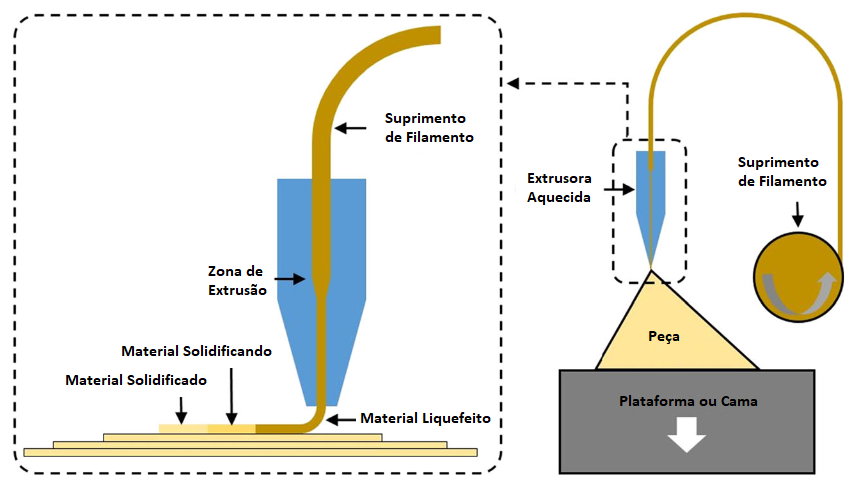
\includegraphics[width=0.7\textwidth]{bikas2015FDM}

    {\footnotesize Fonte:Adaptado de \citeauthor{bikas16}, \citeyear{bikas16}}
    \label{fig:fdm_ex}
    \end{center}
\end{figure}
\end{frame}

\begin{frame}
  \frametitle{\insertsubsection}
  \begin{figure}[H]
    \centering
    \caption{Indicação dos componentes de uma impressora 3D}
    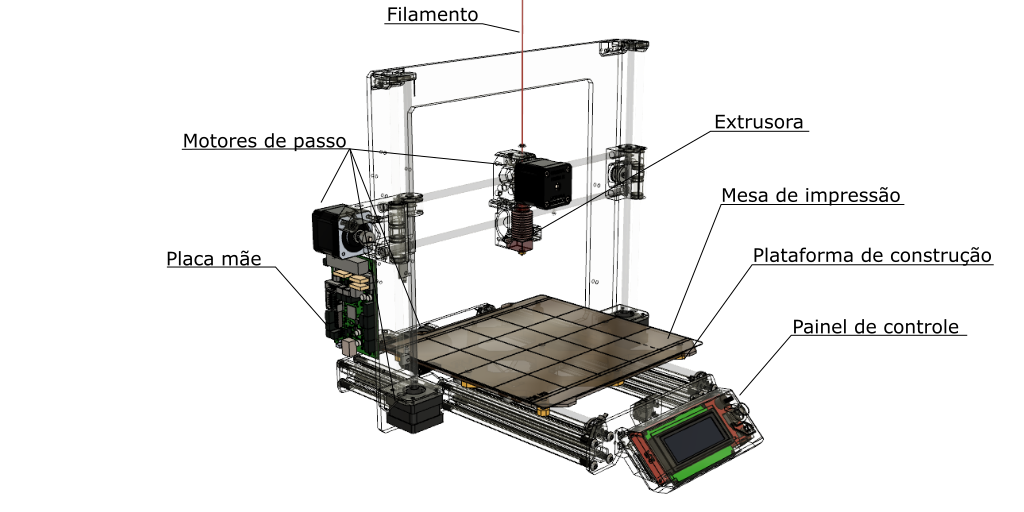
\includegraphics[width=0.8\textwidth]{printer_components}
    \label{fig:impressora3d_comp}
  \end{figure}
\end{frame}

\subsection{\insertsectionnumber .\insertsubsectionnumber . Geração do Modelo 3D digital}
\begin{frame}
  \frametitle{\insertsubsection}
  \begin{itemize}
    \item \textit{Computer Aided Design} (CAD)
    \item Escultura digital
    \item Escaneamento 3D
  \end{itemize}
\end{frame}

\subsection{\insertsectionnumber .\insertsubsectionnumber . Geração de Comando}
\begin{frame}
  \frametitle{\insertsubsection}
  \begin{figure}[H]
    \centering
    \caption{Interface do fatiador PrusaSlicer}
    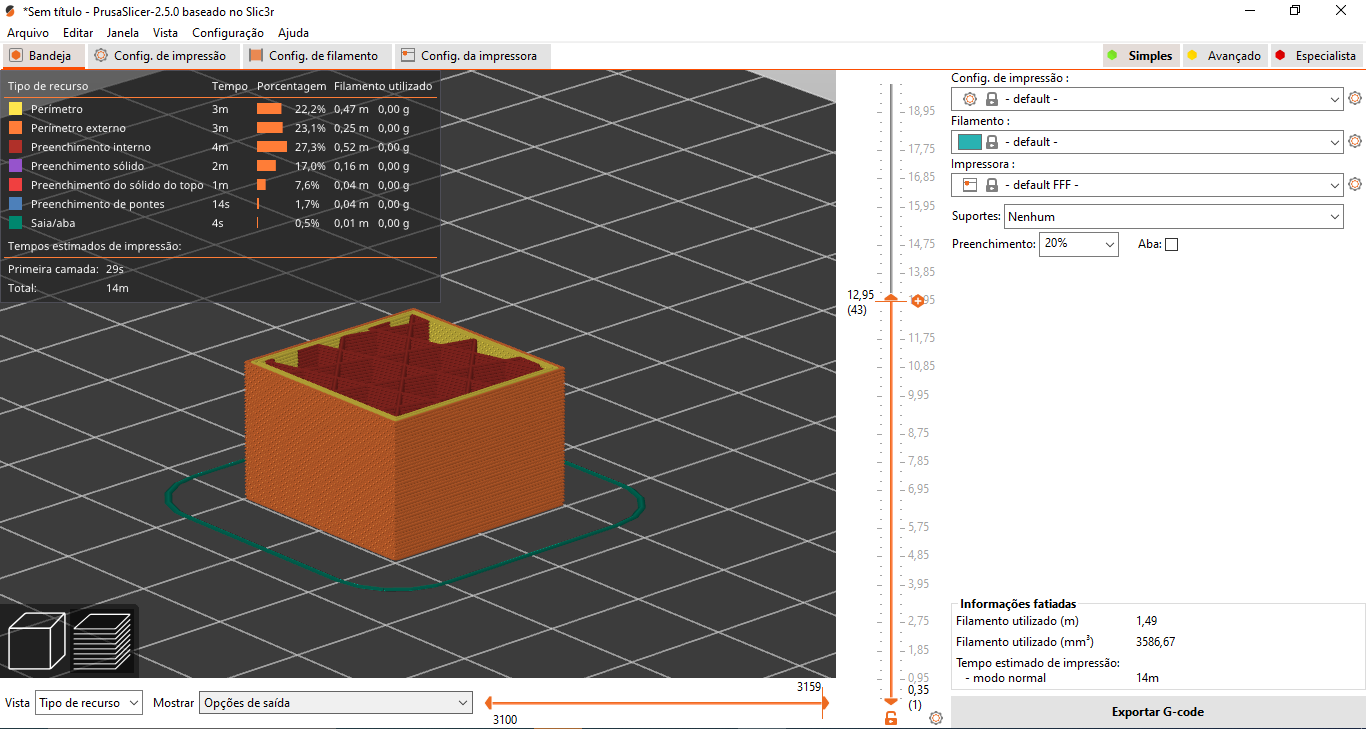
\includegraphics[width=0.8\textwidth]{slicer_inter}
    \label{fig:slicer_inter}
  \end{figure}
\end{frame}

\begin{frame}
  \frametitle{\insertsubsection}
  Exemplos de comandos Gcode
  \begin{itemize}
    \item G090
    \item G1 Y10 F1300
    \item G1 X10 Y5 Z0.2 E1.5 F3000
    \item 
  \end{itemize}
\end{frame}

\subsection{\insertsectionnumber .\insertsubsectionnumber . Geração de Trajetória}
\begin{frame}
  \frametitle{\insertsubsection}
  \begin{figure}[H]
    \centering
    \caption{Perfil de velocidade - Curva trapezoidal de velocidade}
    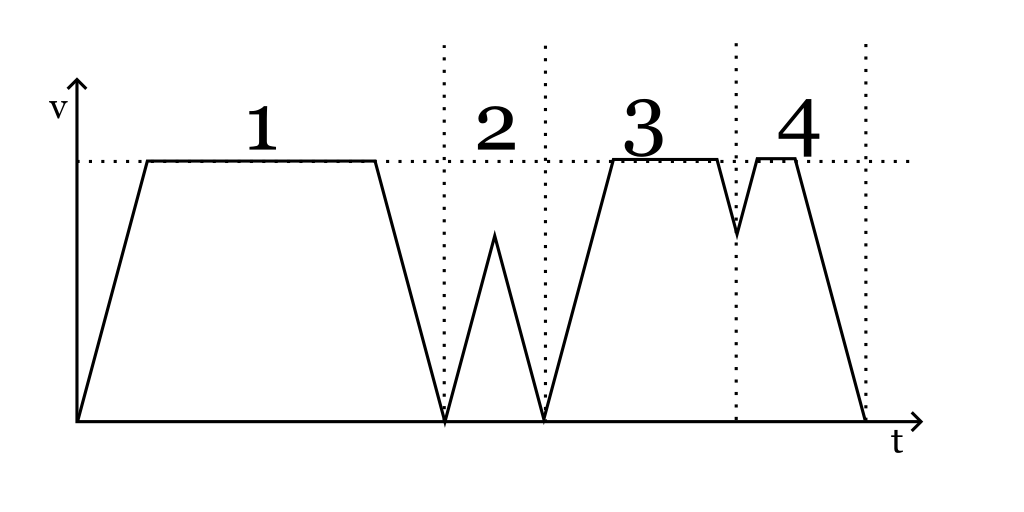
\includegraphics[scale=0.5]{trap_triang}
    \label{fig:trap_triang}
  \end{figure}
\end{frame}

\subsection{\insertsectionnumber .\insertsubsectionnumber . Controle Feedforward}
\begin{frame}
  \frametitle{\insertsubsection}
  \begin{itemize}
    \item Não se faz necessário adcionar sensores e componentes caros
    \item Possui uma característica preditiva ao inves de corretiva
    \item Bons resultados para modelos representativos do sistema real
  \end{itemize}
\end{frame}

\subsection{\insertsectionnumber .\insertsubsectionnumber . \textit{Input Shaping}}
\begin{frame}
  \frametitle{\insertsubsection}
  \begin{figure}[H]
    \centering
    \caption{Comparação da resposta ao degrau e da resposta a escada}
    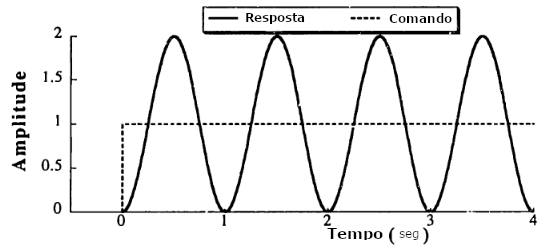
\includegraphics[width=0.45\textwidth]{inputshaperstepresponse1order}
    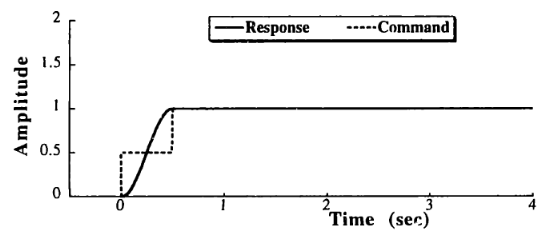
\includegraphics[width=0.45\textwidth]{inputshaperstarcasepresponse}

    {\footnotesize Fonte: Adaptado de \citeauthor{singhose97}, \citeyear{singhose97}}
    \label{fig:degr_vs_esc}
  \end{figure}
\end{frame}

%Conceitos importantes para metodos de controle%

\subsection{\insertsectionnumber .\insertsubsectionnumber . Espaço de Estados}

\begin{frame}
  \frametitle{\insertsubsection}

    \begin{equation}
      \label{eq:edo_ex}
      m \ddot x+c \dot x+kx = f(t)
  \end{equation}

  \begin{equation}
      \label{eq:espaco_de_estados_ex}
      \begin{bmatrix}
          \dot x \\
          \ddot x
      \end{bmatrix}
      =
      \begin{bmatrix}
          0 & 1 \\
          k/m & c/m
      \end{bmatrix}
      \begin{bmatrix}
          x \\
          \dot x
      \end{bmatrix}
      +
      \begin{bmatrix}
          0 \\
          1
      \end{bmatrix}
      f(t)
  \end{equation}
\end{frame}

\subsection{\insertsectionnumber .\insertsubsectionnumber . Programação não linear}

\begin{frame}
  \frametitle{\insertsubsection}

  \begin{columns}
    \begin{column}{.6\textwidth}
      \begin{figure}[H]
        \centering
        \caption{Ilustração Segmentação Cúbica}
        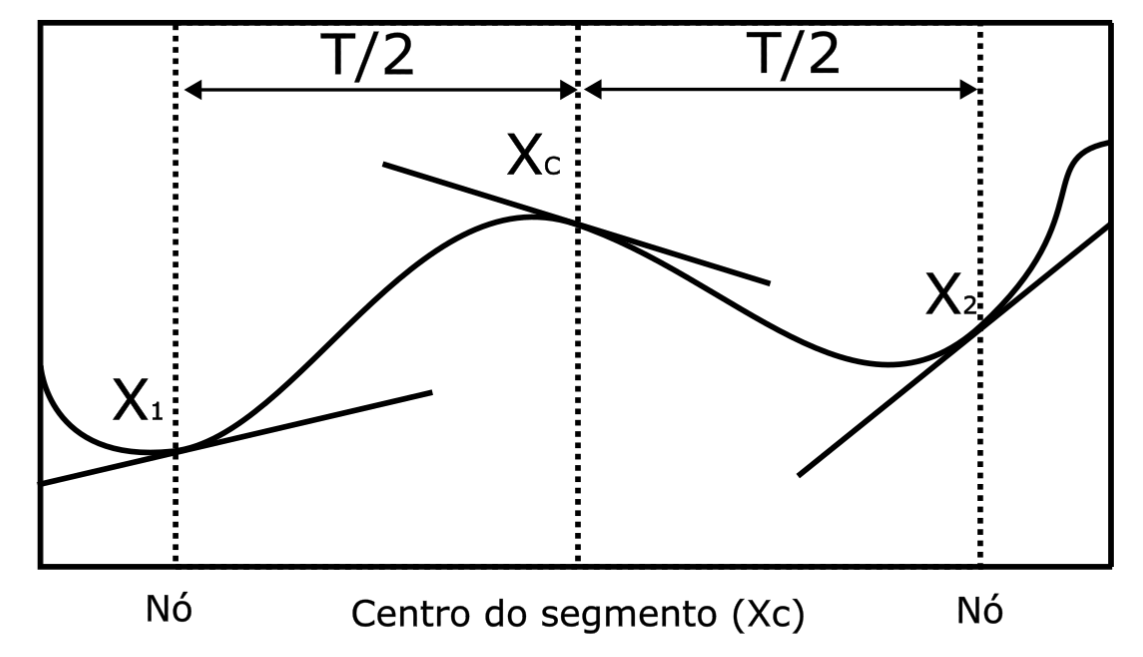
\includegraphics[width=1\textwidth]{hargraves_func}
    
        {\footnotesize Fonte: Adaptado de \citeauthor{hargraves87}, \citeyear{hargraves87}}
        \label{fig:hargraves_fun}
      \end{figure}
    \end{column}
    \begin{column}{.45\textwidth}
      \begin{equation}
        \label{eq:state_center_segment}
        x_c = \frac{x_{1} + x_{2}}{2} + T\frac{f_{1} - f_{2}}{8}
      \end{equation}
    
      \begin{equation}
        \label{eq:state_dot_center_segment}
        \dot{x_{c}} = -3\frac{x_{1} + x_{2}}{2T} + \frac{f_{1} + f_{2}}{4}
      \end{equation}
    
      \begin{equation}
        \label{eq:defect_calc}
        \Delta = f_c - \dot{x_c}
      \end{equation}
    
      \begin{equation}
        \label{eq:input_value_center_segment}
        u_c = \frac{u_1 + u_2}{2}
      \end{equation}
    \end{column}
  \end{columns}
\end{frame}

\section{\insertsectionnumber . Metodologia}
\begin{frame}
  \frametitle{\insertsection}
  \begin{figure}[H]
    \centering
    \caption{Fluxograma geral das etapas para o controle de trajetória}
    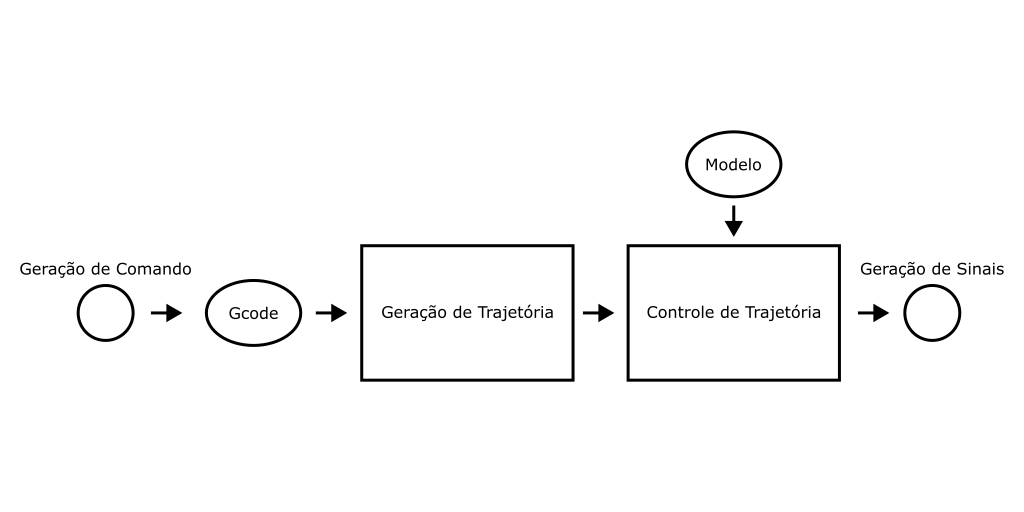
\includegraphics[width=.9\textwidth]{fluxo_geral}
  
    \label{fig:fluxo_geral}
  \end{figure}
\end{frame}

\subsection{\insertsectionnumber .\insertsubsectionnumber . Geração de Trajetória}

\begin{frame}
  \frametitle{\insertsubsection}
  \begin{figure}[H]
    \centering
    \caption{Curva de velocidade trapezoidal}
    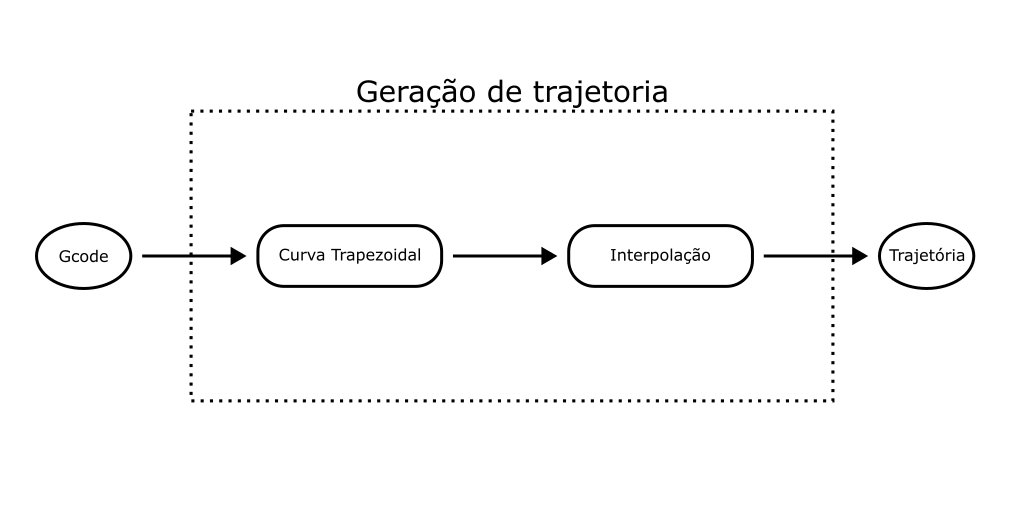
\includegraphics[width=.9\textwidth]{geracao_de_trajetoria}

    \label{fig:geracao_de_trajetoria}
  \end{figure}
\end{frame}

\begin{frame}
  \frametitle{\insertsubsection}
  \begin{columns}
    \begin{column}{.5\textwidth}
      \begin{figure}[H]
        \centering
        \caption{Curva de velocidade triangular}
        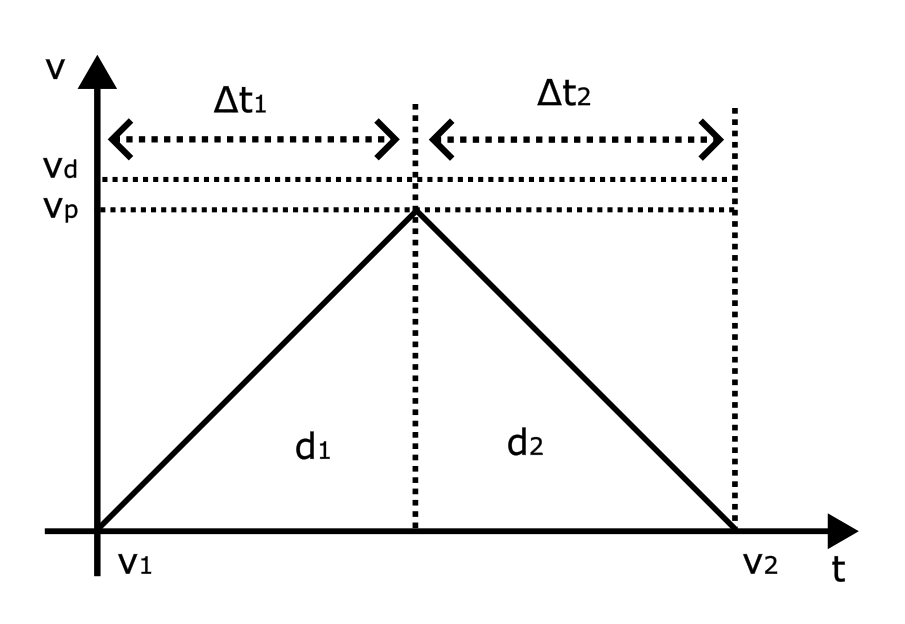
\includegraphics[width=1\textwidth]{triang_curv}

        \label{fig:triang_curv}
      \end{figure}
    \end{column}
    \begin{column}{.45\textwidth}
      \begin{equation}
        \label{eq:v_p}
        v_p = \sqrt{\frac{(v_1^2+v_2^2)}{2}+a d}
      \end{equation}
      \begin{equation}
        \label{eq:des_seg_1_tri}
        d_1 = \frac{(v_p^2-v_1^2)}{(2 a)}
      \end{equation}
      
      \begin{equation}
        \label{eq:des_seg_2_tri}
        d_2 = \frac{(v_2^2-v_p^2)}{(2 a)}
      \end{equation}
      
      \begin{equation}
        \label{eq:dt_seg_1_tri}
        t_1 = \frac{(v_p-v_1)}{a}
      \end{equation}
      
      \begin{equation}
        \label{eq:dt_seg_2_tri}
        t_2 = \frac{(v_2-v_p)}{a}
      \end{equation}
    \end{column}
  \end{columns}
\end{frame}

\begin{frame}
  \frametitle{\insertsubsection}
  \begin{figure}[H]
    \centering
    \caption{Curva de velocidade trapezoidal}
    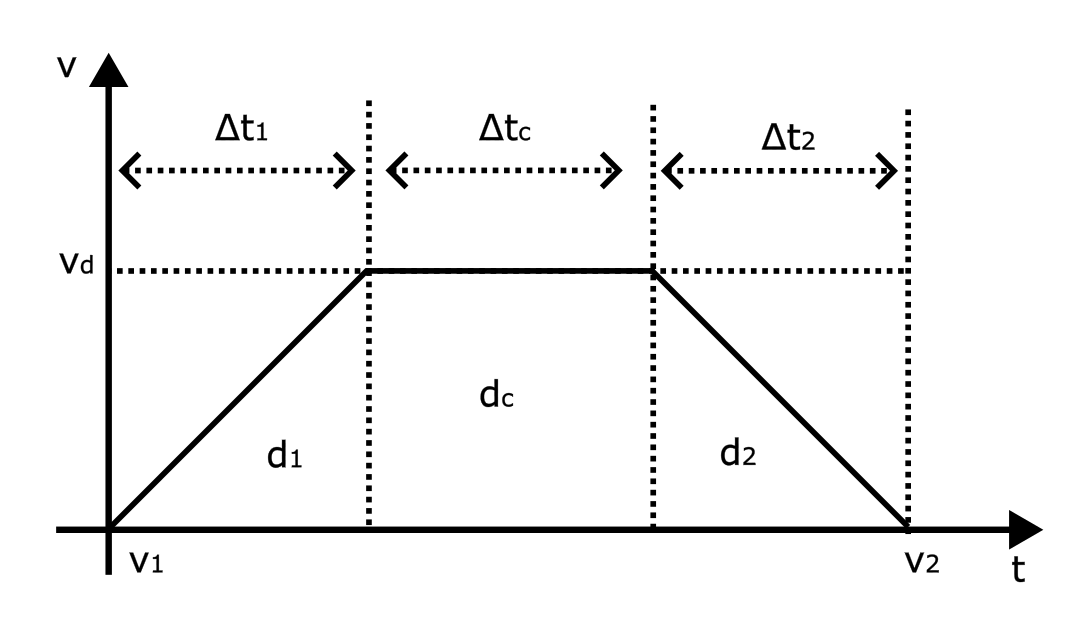
\includegraphics[width=.8\textwidth]{trap_curv}
    \label{fig:trap_curv}
  \end{figure}
\end{frame}

\begin{frame}
  \frametitle{\insertsubsection}
  \begin{columns}
    \begin{column}{.45\textwidth}
      
      \begin{equation}
        \label{eq:des_seg_1_trap}
        d_1 = \frac{(v_d^2-v_1^2)}{(2 a)}
      \end{equation}

      \begin{equation}
        \label{eq:des_seg_2_trap}
        d_2 = \frac{(v_2^2-v_d^2)}{(2 a)}
      \end{equation}

      \begin{equation}
        \label{eq:des_seg_c_trap}
        d_c = d-(d_1+d_2)
      \end{equation}
    \end{column}
    \begin{column}{.45\textwidth}
      
      \begin{equation}
        \label{eq:dt_seg_1_trap}
        \Delta t_1 = \frac{(v_d-v_1)}{a}
      \end{equation}

      \begin{equation}
        \label{eq:dt_seg_2_trap}
        \Delta t_2 = \frac{(v_2-v_d)}{a}
      \end{equation}

      \begin{equation}
        \label{eq:dt_seg_c_trap}
        \Delta t_c = \frac{d_c}{v_d}
      \end{equation}
    \end{column}
  \end{columns}
\end{frame}

\subsection{\insertsectionnumber .\insertsubsectionnumber . Modelagem Dinâmica de uma Impressora 3D}

\begin{frame}
  \frametitle{\insertsubsection}
  \begin{itemize}
    \item Influência da Correia: A correia é o componente chave responsável por introduzir desvios nas trajetórias de impressão. Ela age como uma combinação de mola e amortecedor, afetando a dinâmica do movimento.
    \item Modelagem do Conjunto Bico Injetor e Extrusora: Este conjunto é tratado como um corpo rígido uniforme, simplificando sua representação geométrica.
    \item Dimensões da Mesa de Impressão: A área útil da mesa de impressão é de 200 mm x 200 mm, definindo o espaço de trabalho disponível.
    \item Configuração Cartesiana: A impressora opera em um sistema cartesiano, com eixos ortogonais, o que simplifica a análise de movimento.
    \item Independência dos Eixos: Cada eixo da impressora opera independentemente dos outros, permitindo uma análise mais simplificada das dinâmicas individuais.
    \item Condições Iniciais de Movimento: Assume-se que todos os movimentos da impressora iniciam a partir do estado de repouso.
\end{itemize}
\end{frame}

\begin{frame}
  \frametitle{\insertsubsection}
  \begin{figure}[H]
    \centering
    \caption{Modelo simplificado impressora 3D}
    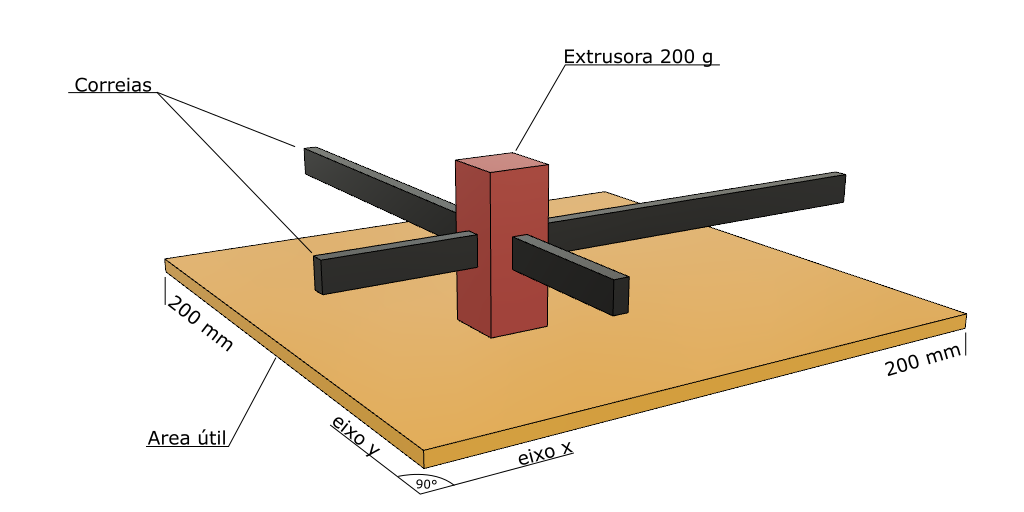
\includegraphics[width=0.6\textwidth]{simple_model}
    \label{fig:simple_model}
  \end{figure}
\end{frame}

\begin{frame}
  \frametitle{\insertsubsection}
  \begin{equation}
    \label{eq:mov_impressora_2}
    \ddot{x_p} = \frac{c}{m}(\dot{x_b} - \dot{x_p}) + \frac{k}{m}(x_b - x_p) 
  \end{equation}
  \begin{figure}[H]
    \centering
    \caption{Modelagem de 1 eixo}
    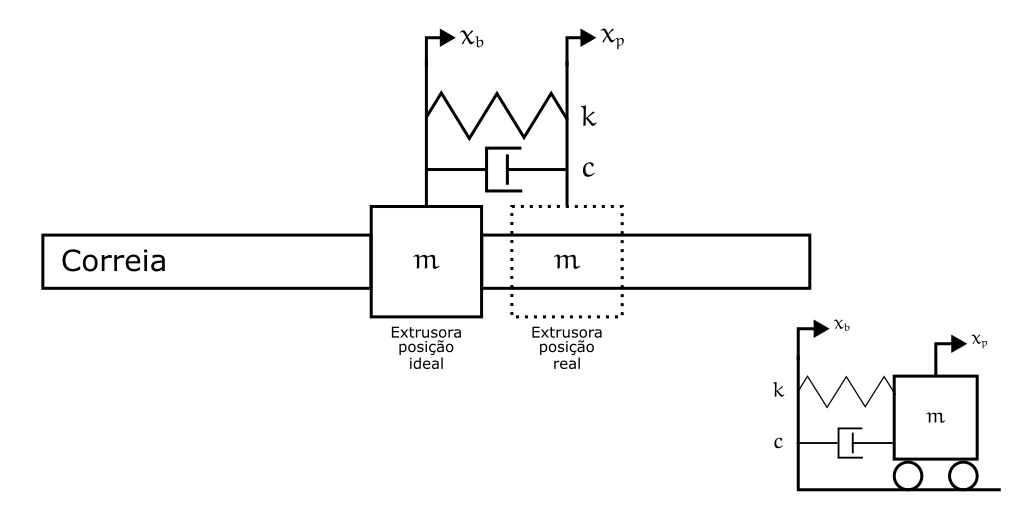
\includegraphics[width=.7\textwidth]{model_1_axis}

    \label{fig:model_1_axis}
  \end{figure}
\end{frame}

\begin{frame}
  \frametitle{\insertsubsection}
  \begin{figure}[H]
    \centering
    \caption{Modelagem dos eixos x e y}
    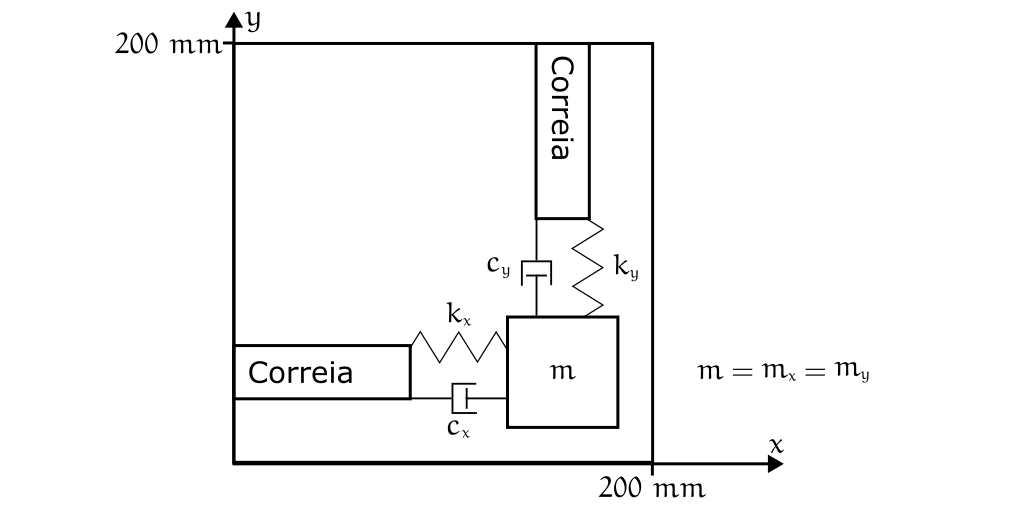
\includegraphics[scale=0.4]{model_2_axis}

    \label{fig:model_2_axis}
  \end{figure}
\end{frame}

\begin{frame}
  \frametitle{\insertsubsection}
  
  \begin{equation}
    \label{eq:freq_nat}
    \omega = \sqrt{\frac{k}{m}}
  \end{equation}
  
  \begin{equation}
    \label{eq:amort}
    \zeta = \frac{c}{2mk}
  \end{equation}
  
  \begin{equation}
    \label{eq:equation_simpl}
    \ddot{x_p} = 2 \zeta \omega(\dot{x_b} - \dot{x_p}) + \omega ^2(x_b - x_p)
  \end{equation}
\end{frame}

\subsection{\insertsectionnumber .\insertsubsectionnumber . Representação em Espaço de Estados}
\begin{frame}
  \frametitle{\insertsubsection}
  \begin{equation}
    \label{eq:simp_state_space_din_model}
    \dot x = A*x+B*u
  \end{equation}
  
  \begin{equation}
    \label{eq:espaco_de_estados_din_model}
    \begin{bmatrix}
        \dot{x_p} \\
        \dot{y_p} \\
        \ddot{x_p} \\
        \ddot{y_p}
    \end{bmatrix}
    =
    \begin{bmatrix}
        0 & 0 & 1 & 0 \\
        0 & 0 & 0 & 1 \\
        -\omega _x ^2 & 0 & -2 \zeta _x \omega _x & 0 \\
        0 & -\omega _y ^2 & 0 & -2 \zeta _y \omega _y
    \end{bmatrix}
    \begin{bmatrix}
        x_p \\    
        y_p \\
        \dot{x_p} \\    
        \dot{y_p} \\
    \end{bmatrix}
    +
    \begin{bmatrix}
        0 & 0 & 0 & 0 \\
        0 & 0 & 0 & 0 \\
        \omega _x ^2 & 0 & 2 \zeta _x \omega _x & 0 \\
        0 & \omega _y ^2 & 0 & 2 \zeta _y \omega _y
    \end{bmatrix}
    \begin{bmatrix}
        x_b \\
        y_b \\
        \dot{x_b}  \\
        \dot{y_b} 
    \end{bmatrix}
  \end{equation}
\end{frame}

\subsection{\insertsectionnumber .\insertsubsectionnumber . Controle de Trajetória}
\begin{frame}
  \frametitle{\insertsubsection}
  \begin{figure}[H]
    \centering
    \caption{Fluxograma Controle de Trajetória}
    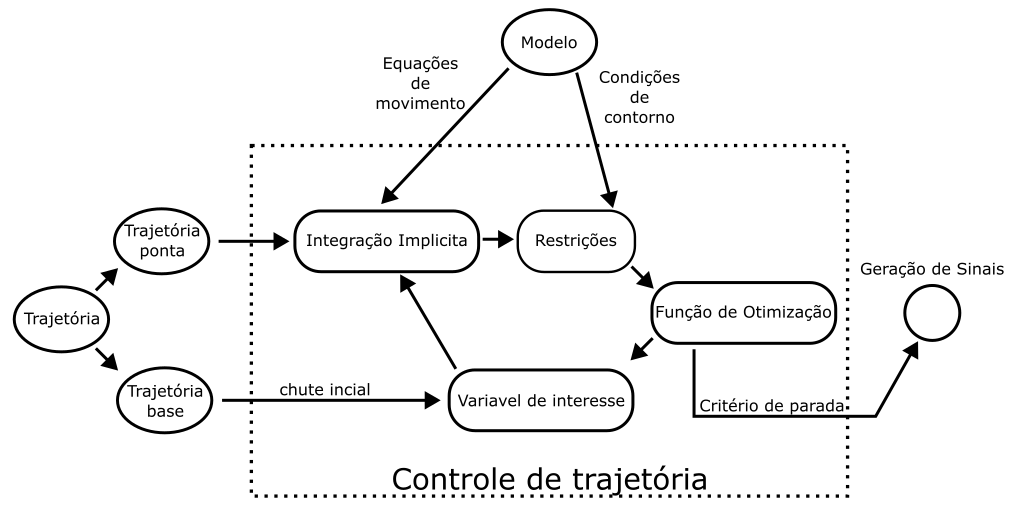
\includegraphics[scale=0.5]{controle_de_trajetoria}

    \label{fig:controle_de_trajetoria}
  \end{figure}
\end{frame}

\subsection{\insertsectionnumber .\insertsubsectionnumber . Restrições}
\begin{frame}
  \frametitle{\insertsubsection}
  \begin{itemize}
    \item 
  \end{itemize}
\end{frame}

\subsection{\insertsectionnumber .\insertsubsectionnumber . Função de otimização}
\begin{frame}
  \frametitle{\insertsubsection}
  \begin{itemize}
    \item 
  \end{itemize}
\end{frame}

\section{\insertsectionnumber . Resultados}

\begin{frame}
  \frametitle{\insertsection}
  \begin{columns}
    \begin{column}{.3\textwidth}
      \begin{itemize}
        \item das
        \item Runge-Kutta
      \end{itemize}
    \end{column}
    \begin{column}{.7\textwidth}
      \begin{figure}[H]
        \centering
        \caption{Movimento base}
        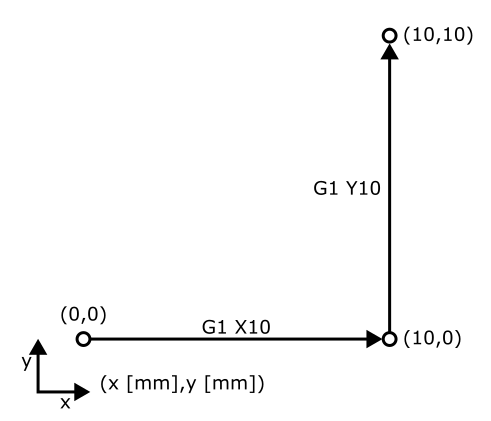
\includegraphics[width=.7\textwidth]{base_mov}
    
        \label{fig:base_mov}
      \end{figure}
    \end{column}
  \end{columns}
\end{frame}

\begin{frame}
  \frametitle{\insertsection}
  \begin{figure}[H]
    \centering
    \caption{Fluxograma geral com os parâmetros.}
    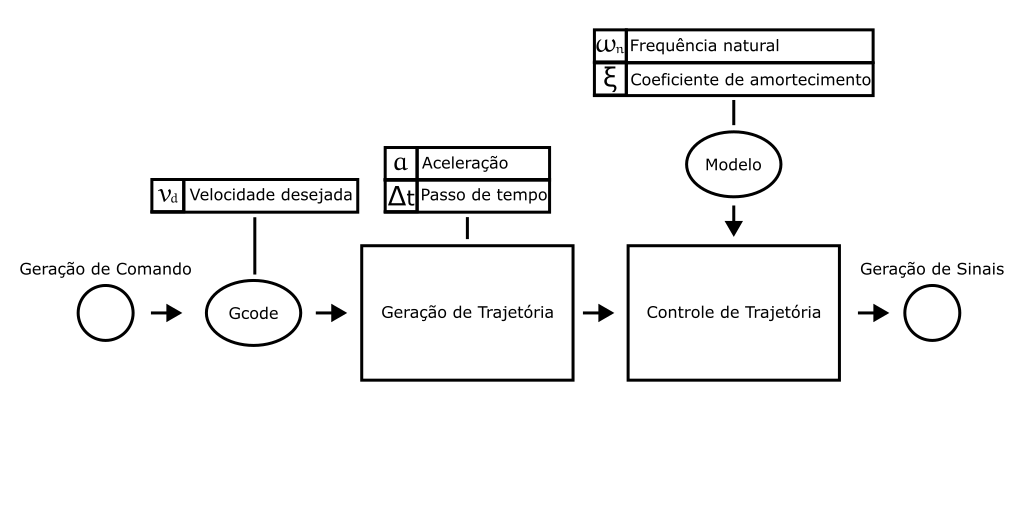
\includegraphics[width=.9\textwidth]{fluxo_geral_var}

    \label{fig:fluxo_geral_var}
\end{figure}
\end{frame}

\subsection{\insertsectionnumber .\insertsubsectionnumber . Simulação Referência}
\begin{frame}
  \frametitle{\insertsubsection}
  \begin{table}
    \begin{center}
    \caption{Valores dos parâmetros utilizados na simulação referência.}
    \label{tab:base_params}
    \begin{tabular}{c c c}
        Parâmetro & Valor & Unidade\\ \hline
        Frequência & 100 & $rad/s$\\
        Coeficiente de amortecimento & 0,5 & - \\
        Aceleração base & 5000 & $mm/s^2$ \\
        Velocidade desejada & 100 & $mm/s$ \\
        Passo de tempo & 0,005 & $s$ \\ \hline
    \end{tabular}
    \end{center}
  \end{table}
\end{frame}

\subsection{\insertsectionnumber .\insertsubsectionnumber . Resultados da Simulação Referência}

\begin{frame}
  \frametitle{\insertsubsection}
  \begin{figure}[H]
    \centering
    \caption{Caminhos da ponta e da base.}
    \subfigure[Sem controle.]{
        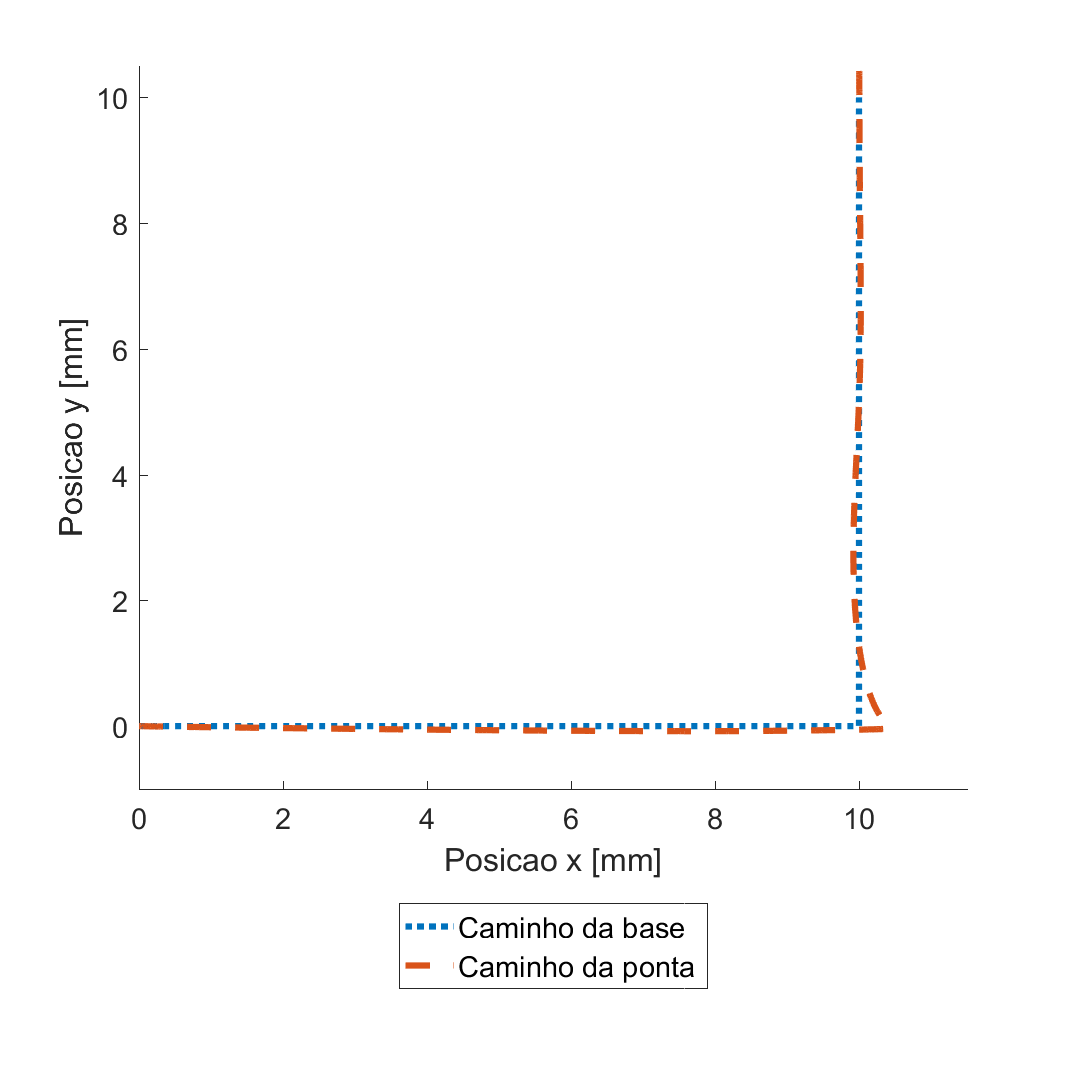
\includegraphics[width=0.38\textwidth]{Sim ref_cam_s.png}
        \label{fig:ref_cam_s}
    }
    \hfill
    \subfigure[Com controle.]{
        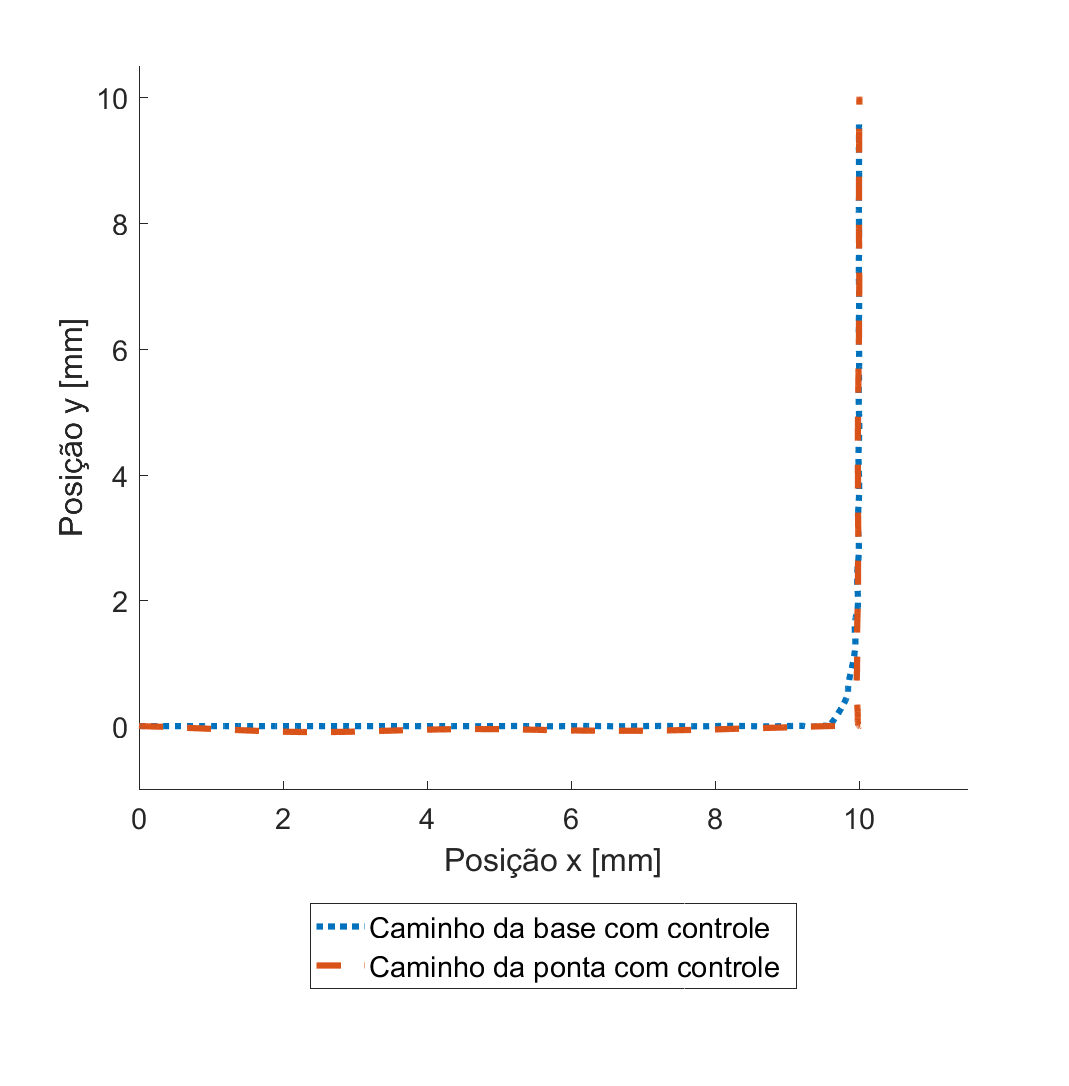
\includegraphics[width=0.38\textwidth]{Sim ref_cam_c.png}
        \label{fig:ref_cam_c}
    }
  \end{figure}
\end{frame}

\begin{frame}
  \frametitle{\insertsubsection}
  \begin{figure}[H]
    \centering
    \caption{Caminhos da ponta e da base - Detalhamento}
    \subfigure[Sem controle.]{
        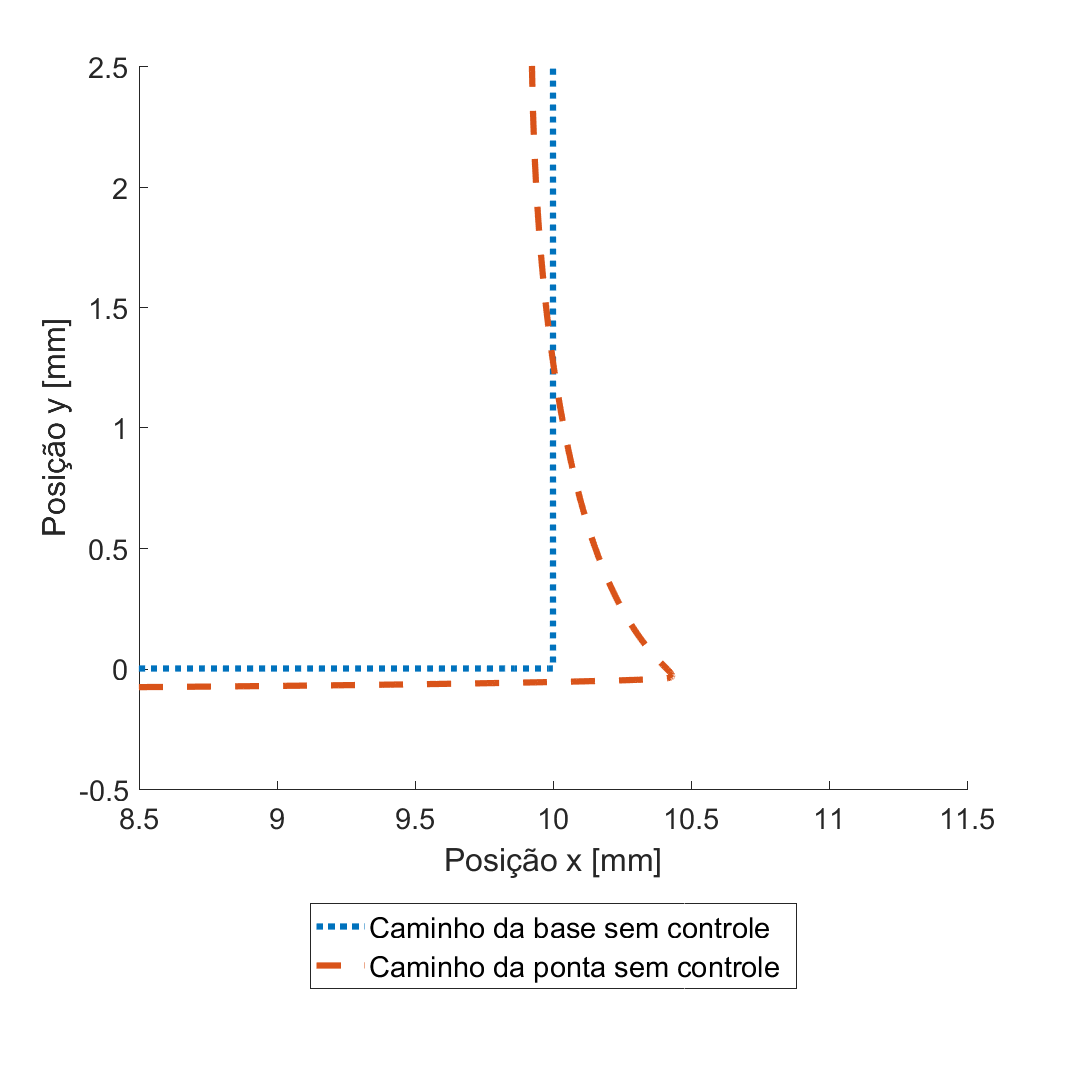
\includegraphics[width=0.38\textwidth]{Sim ref_cam_s_zoom.png}
        \label{fig:ref_cam_s_zoom}
    }
    \hfill
    \subfigure[Com controle.]{
        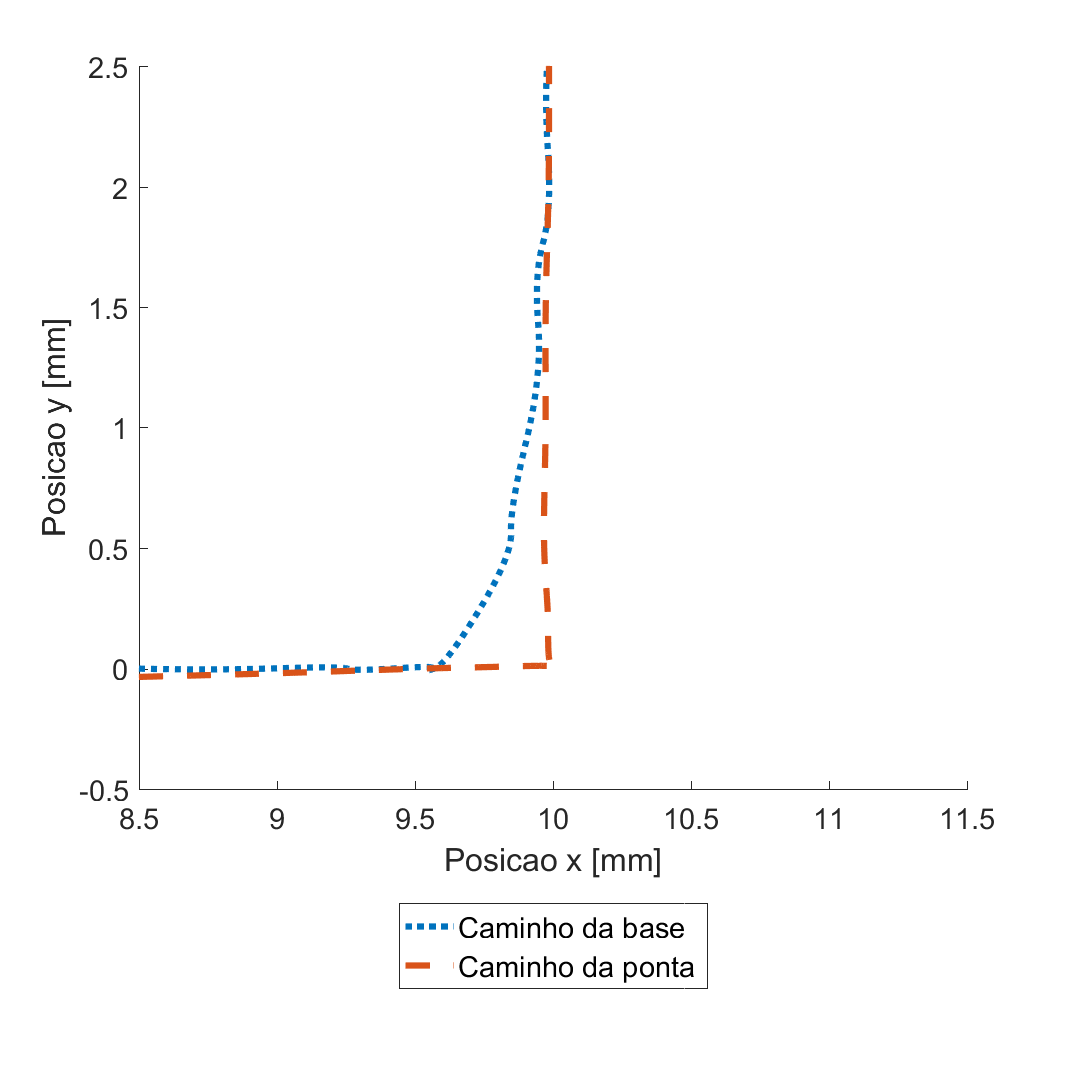
\includegraphics[width=0.38\textwidth]{Sim ref_cam_c_zoom.png}
        \label{fig:ref_cam_c_zoom}
    }
  \end{figure}
\end{frame}

\begin{frame}
  \frametitle{\insertsubsection}
  \begin{figure}[H]
    \centering
    \caption{Deslocamentos da ponta e da base.}
    \subfigure[Sem controle.]{
        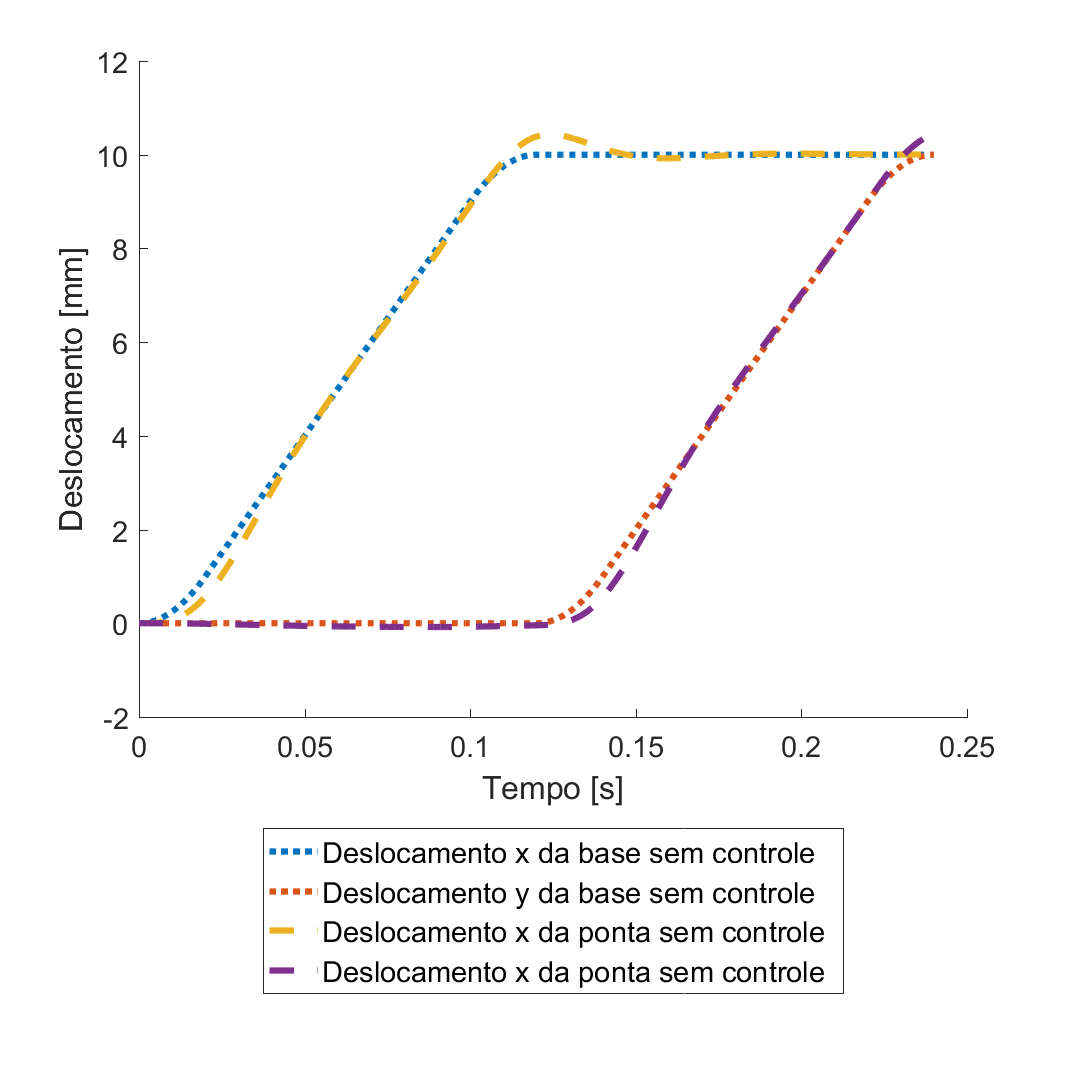
\includegraphics[width=0.38\textwidth]{Sim ref_des_s.png}
        \label{fig:ref_des_s}
    }
    \hfill
    \subfigure[Com controle.]{
        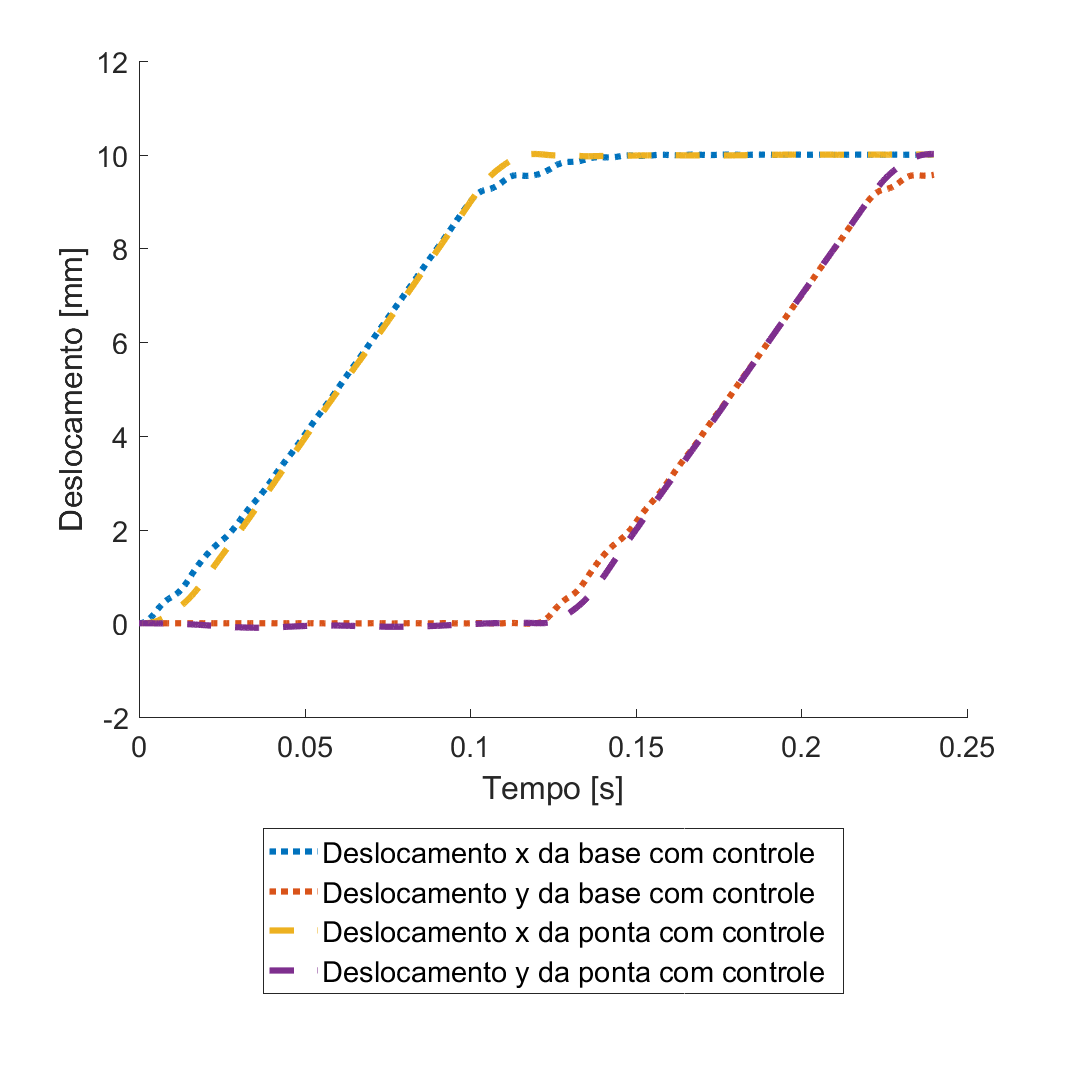
\includegraphics[width=0.38\textwidth]{Sim ref_des_c.png}
        \label{fig:ref_des_c}
    }
    \label{fig:ref_des}
  \end{figure}
\end{frame}

\begin{frame}
  \frametitle{\insertsubsection}
  \begin{figure}[H]
    \centering
    \caption{Velocidades da ponta e da base.}
    \subfigure[Sem controle.]{
        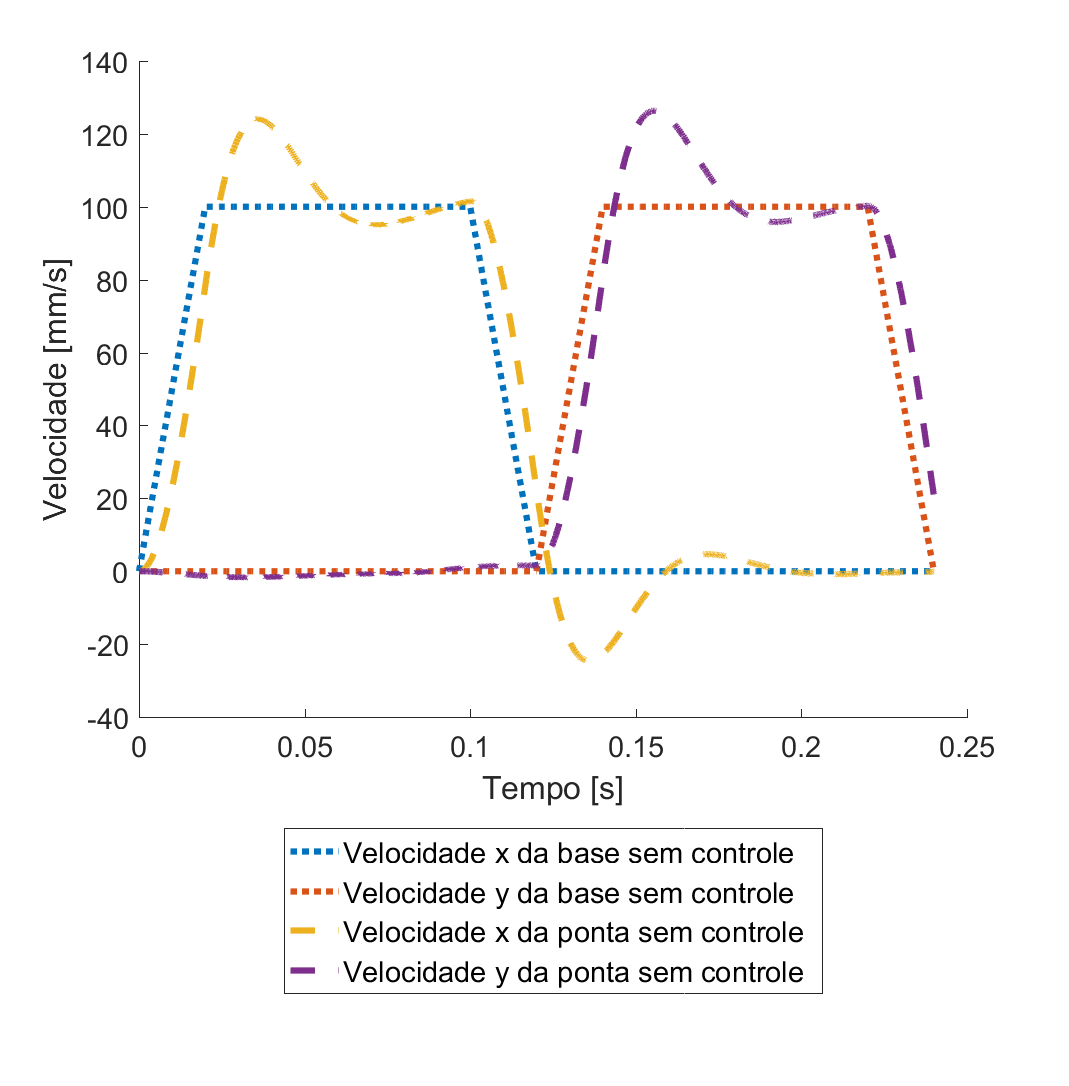
\includegraphics[width=0.38\textwidth]{Sim ref_vel_s.png}
        \label{fig:ref_vel_s}
    }
    \hfill
    \subfigure[Com controle.]{
        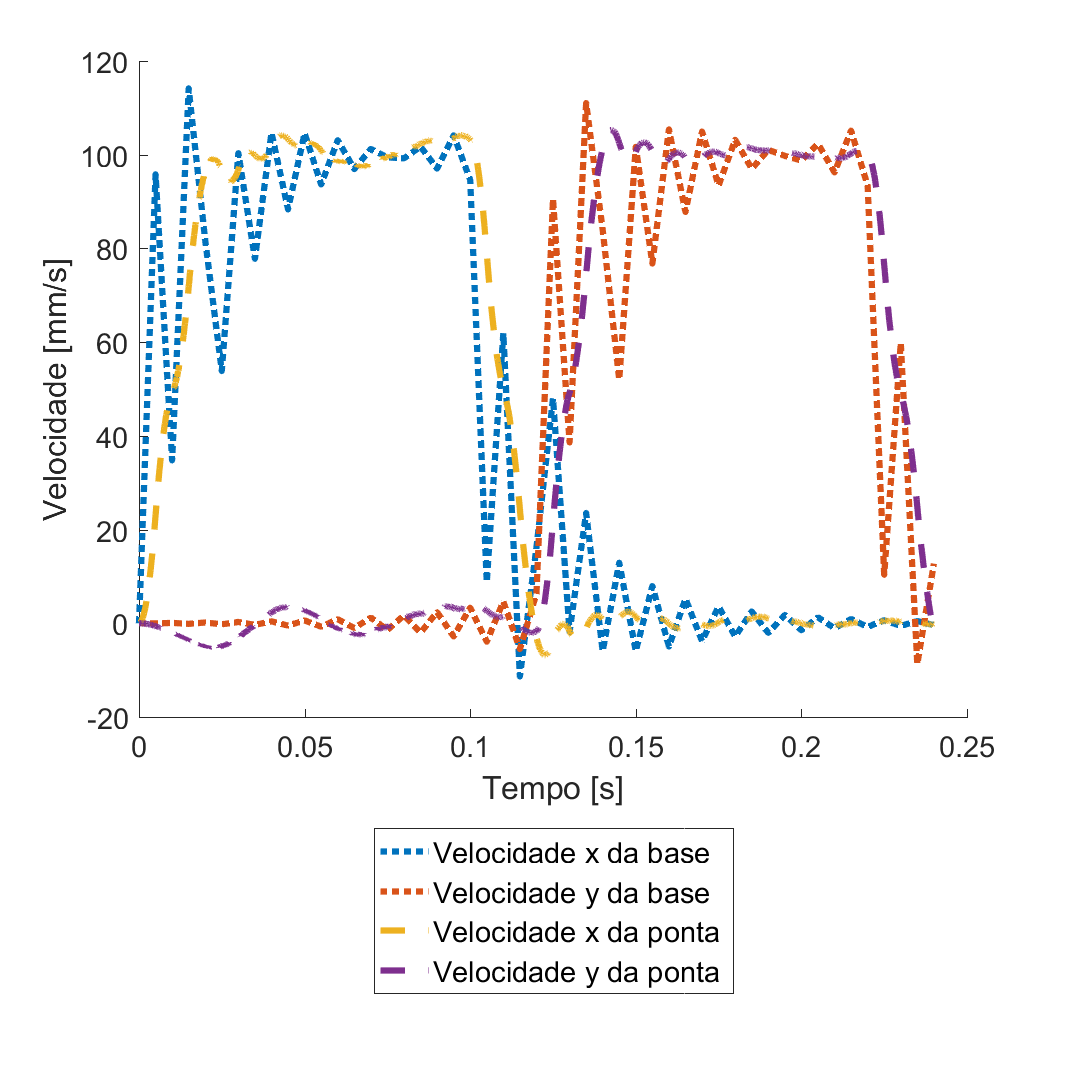
\includegraphics[width=0.38\textwidth]{Sim ref_vel_c.png}
        \label{fig:ref_vel_c}
    }
    \label{fig:ref_vel}
  \end{figure}
\end{frame}

\subsection{\insertsectionnumber .\insertsubsectionnumber . Simulação com Parâmetros Variados}
\begin{frame}
  \frametitle{\insertsubsection}
  \begin{table}
    \begin{center}
    \caption{Parâmetros utilizados nas simulações.}
    \label{tab:sim_params}
    \begin{tabular}{c c c c c}
        Caso & Parâmetro & Valor A & Valor B & Unidade\\ \hline
        1 & Frequência & 50 & 200 & $rad/s$\\
        2 & Coeficiente de amortecimento & 0 & 1 & - \\
        3 & Aceleração base & 1000 & 10000 & $mm/s^2$ \\
        4 & Velocidade desejada & 50 & 200 & $mm/s$ \\
        5 & Passo de tempo & 0,1 & 0,001 & $s$ \\ \hline
    \end{tabular}
    \end{center}
  \end{table}
\end{frame}

\subsection{\insertsectionnumber .\insertsubsectionnumber . Resultados da Simulação - Variação da Frequência Natural}

\begin{frame}
  \frametitle{\insertsubsection}
  \begin{figure}[H]
    \centering
    \caption{Caminhos da ponta e da base - Detalhamento 1A.}
    \subfigure[Detalhamento - Sem controle.]{
        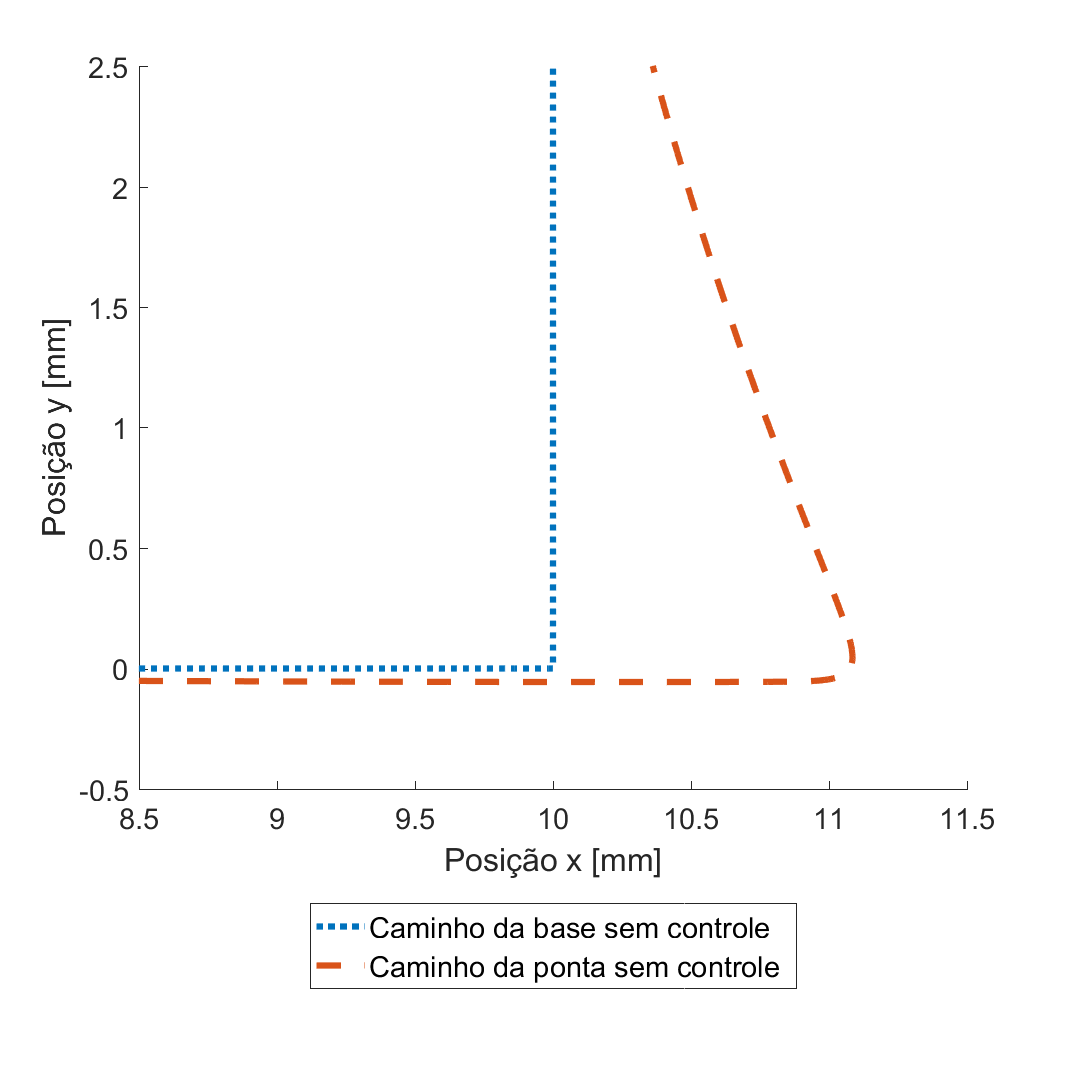
\includegraphics[width=0.38\textwidth]{Sim 1A_cam_s_zoom.png}
        \label{fig:1A_cam_s_zoom}
    }
    \hfill
    \subfigure[Detalhamento - Com controle.]{
        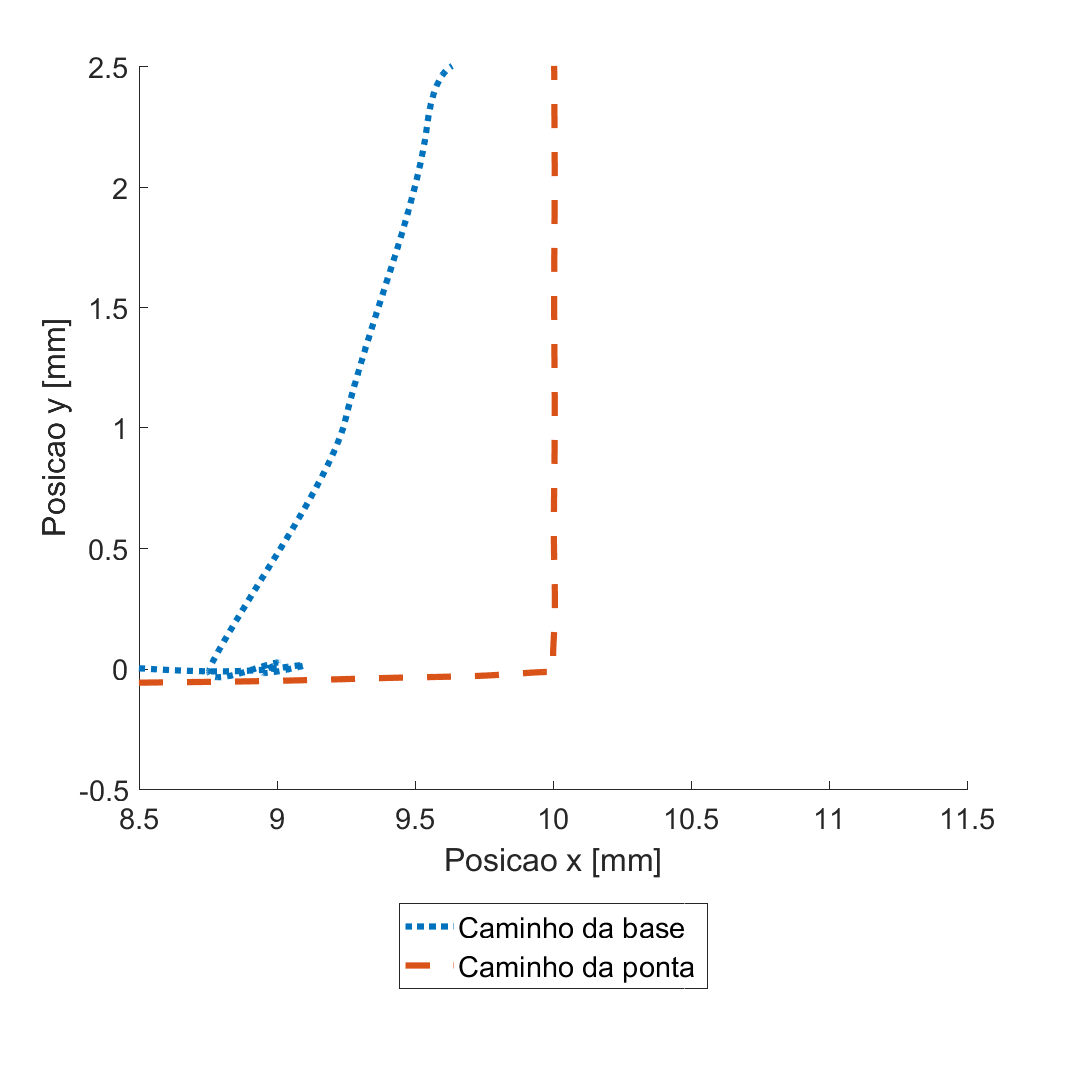
\includegraphics[width=0.38\textwidth]{Sim 1A_cam_c_zoom.png}
        \label{fig:1A_cam_c_zoom}
    }
  \end{figure}
\end{frame}

\begin{frame}
  \frametitle{\insertsubsection}
  \begin{figure}[H]
    \centering
    \caption{Deslocamentos da ponta e da base - Caso 1A.}
    \subfigure[Sem controle.]{
        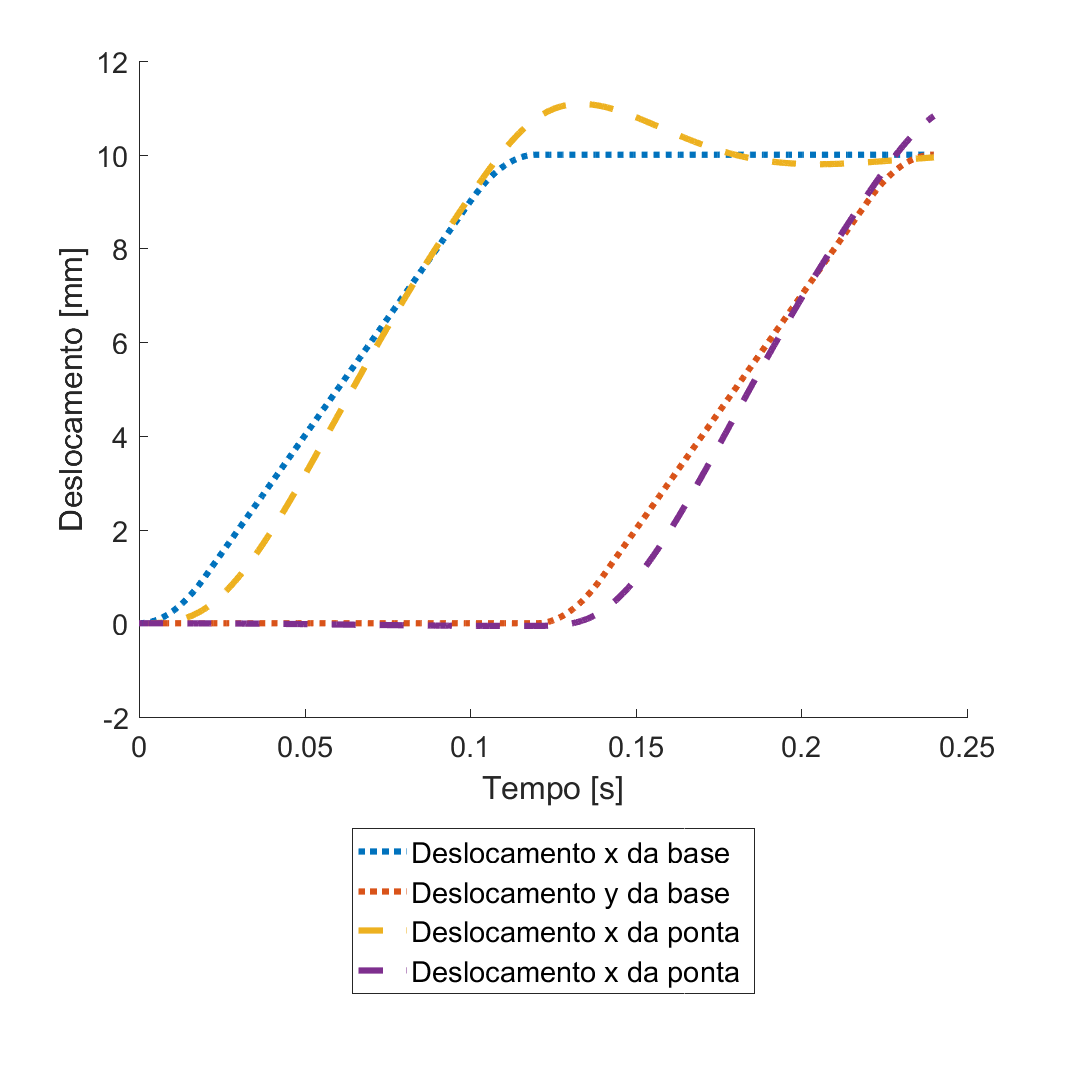
\includegraphics[width=0.38\textwidth]{Sim 1A_des_s.png}
        \label{fig:1A_des_s}
    }
    \hfill
    \subfigure[Com controle.]{
        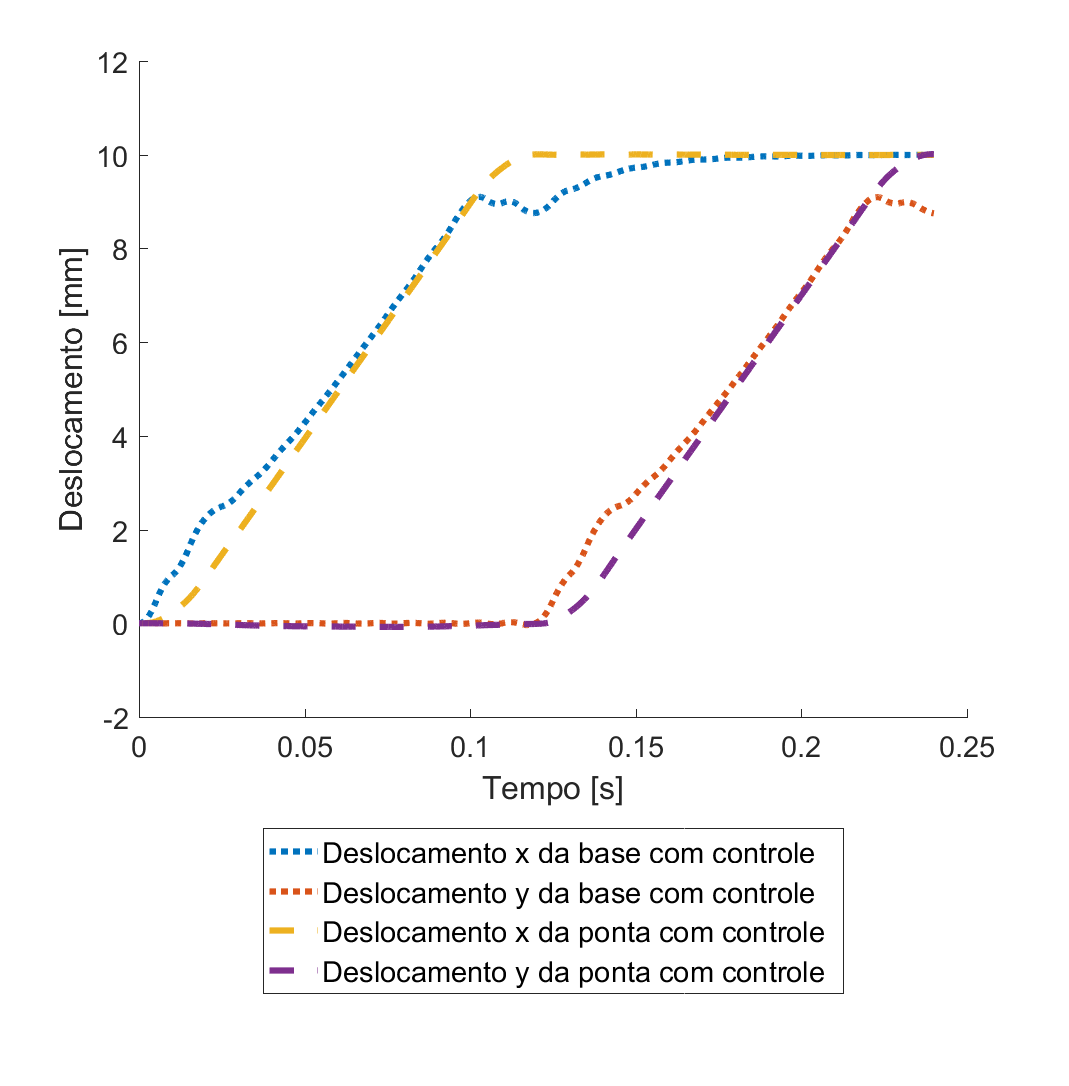
\includegraphics[width=0.38\textwidth]{Sim 1A_des_c.png}
        \label{fig:1A_des_c}
    }
  \end{figure}
\end{frame}

\begin{frame}
  \frametitle{\insertsubsection}
  \begin{figure}[H]
    \centering
    \caption{Caminhos da ponta e da base - Detalhamento 1B}
    \subfigure[Sem controle.]{
        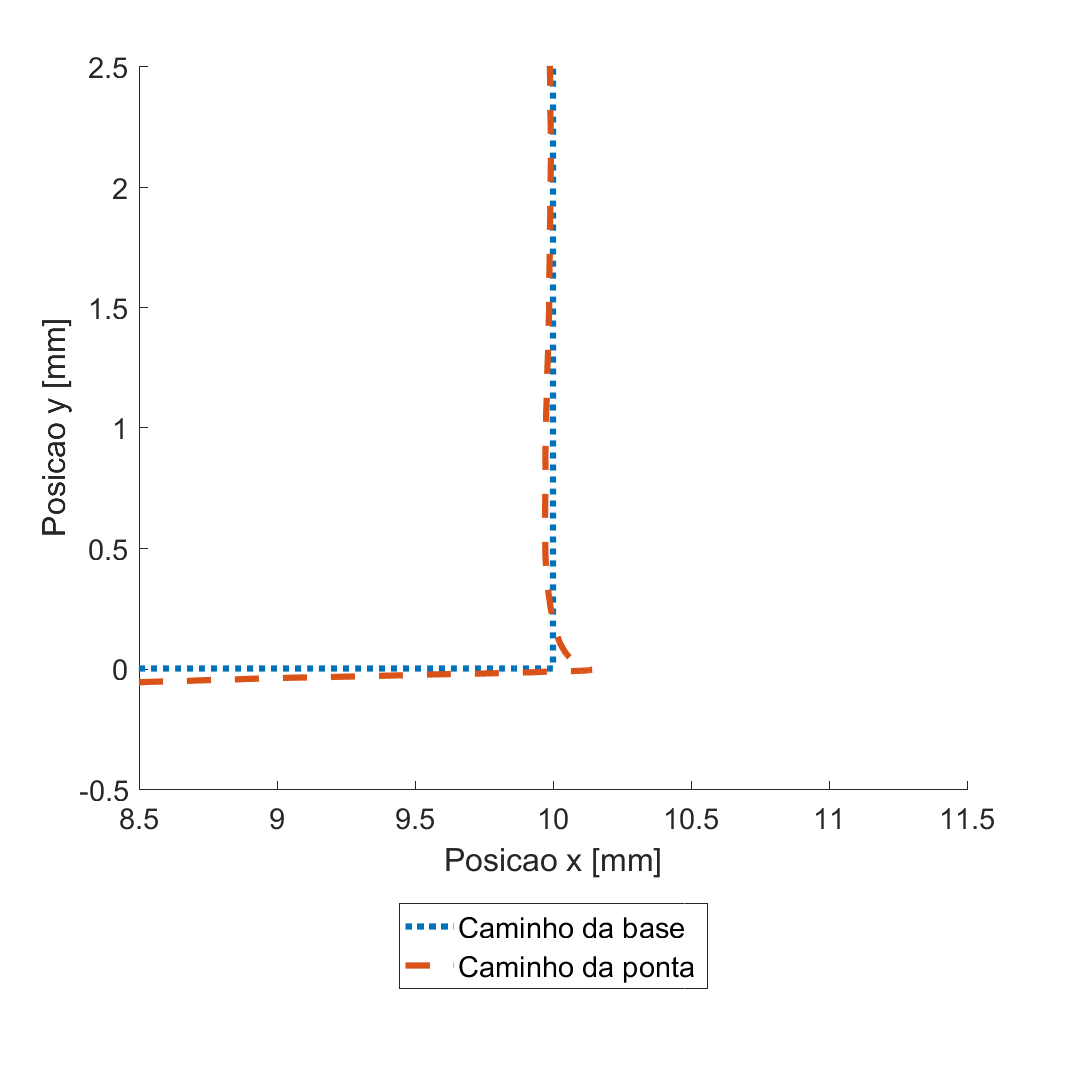
\includegraphics[width=0.38\textwidth]{Sim 1B_cam_s_zoom.png}
        \label{fig:1B_cam_s_zoom}
    }
    \hfill
    \subfigure[Com controle.]{
        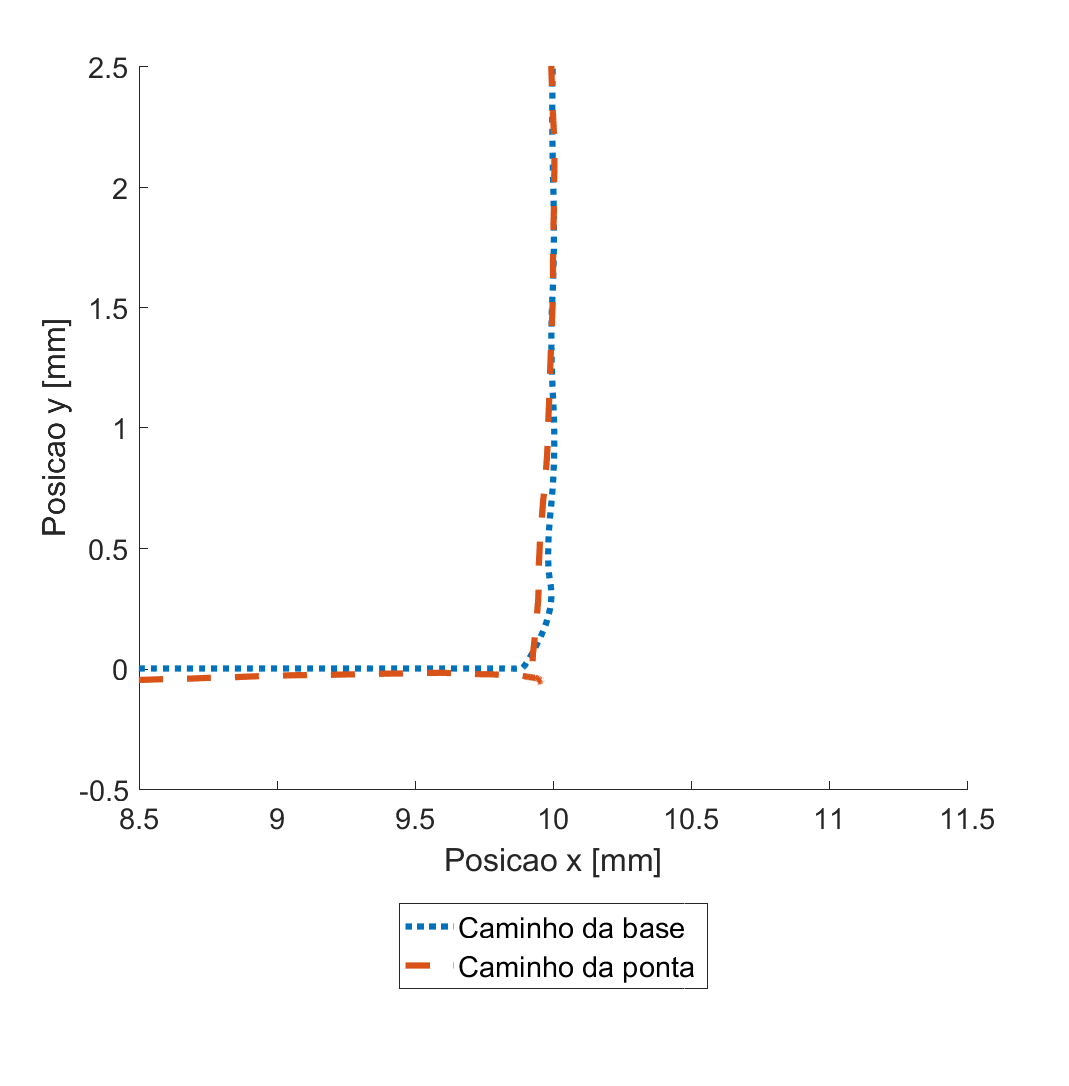
\includegraphics[width=0.38\textwidth]{Sim 1B_cam_c_zoom.png}
        \label{fig:1B_cam_c_zoom}
    }
  \end{figure}
\end{frame}

\begin{frame}
  \frametitle{\insertsubsection}
  \begin{figure}[H]
    \centering
    \caption{Deslocamentos da ponta e da base - Caso 1B.}
    \subfigure[Sem controle.]{
        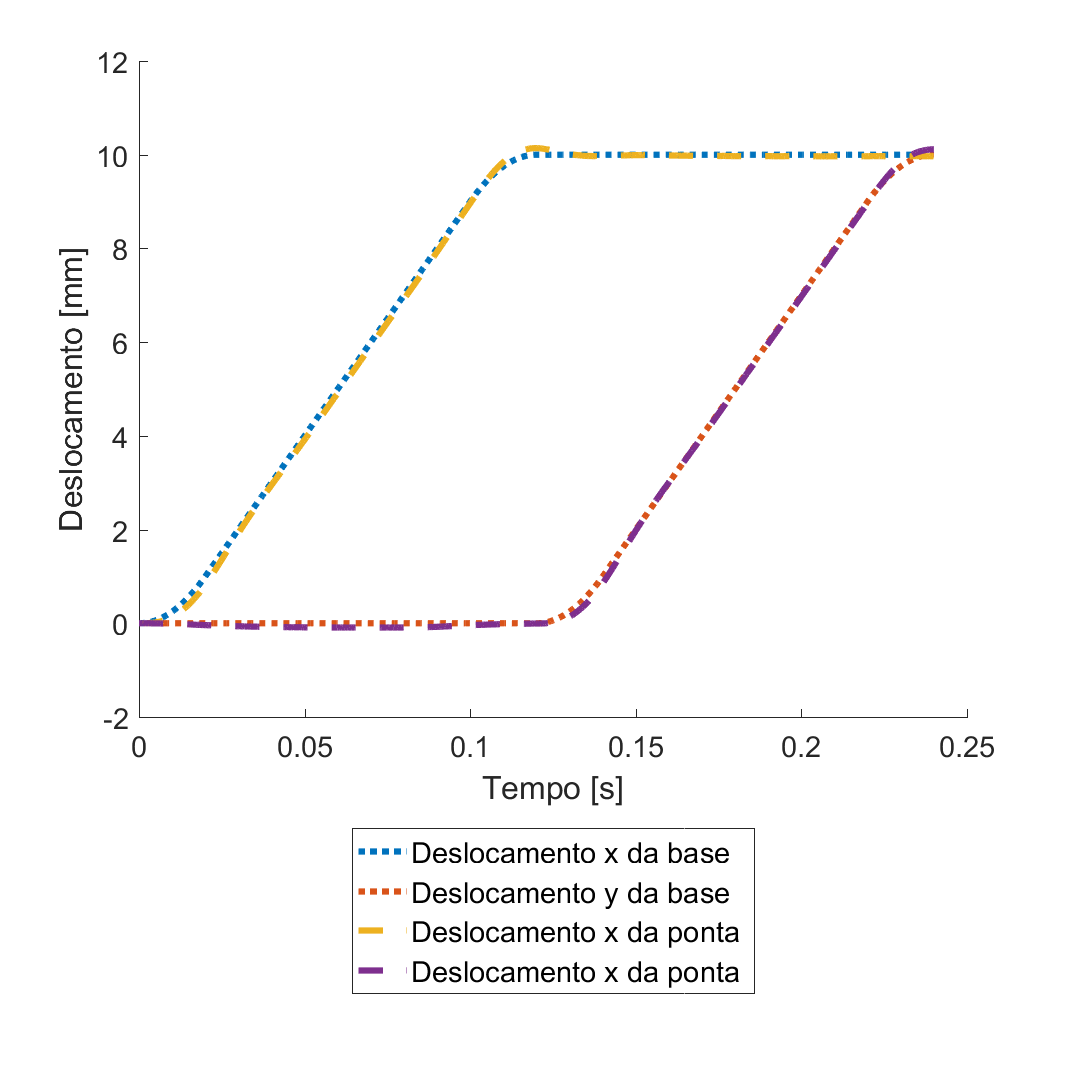
\includegraphics[width=0.38\textwidth]{Sim 1B_des_s.png}
        \label{fig:1B_des_s}
    }
    \hfill
    \subfigure[Com controle.]{
        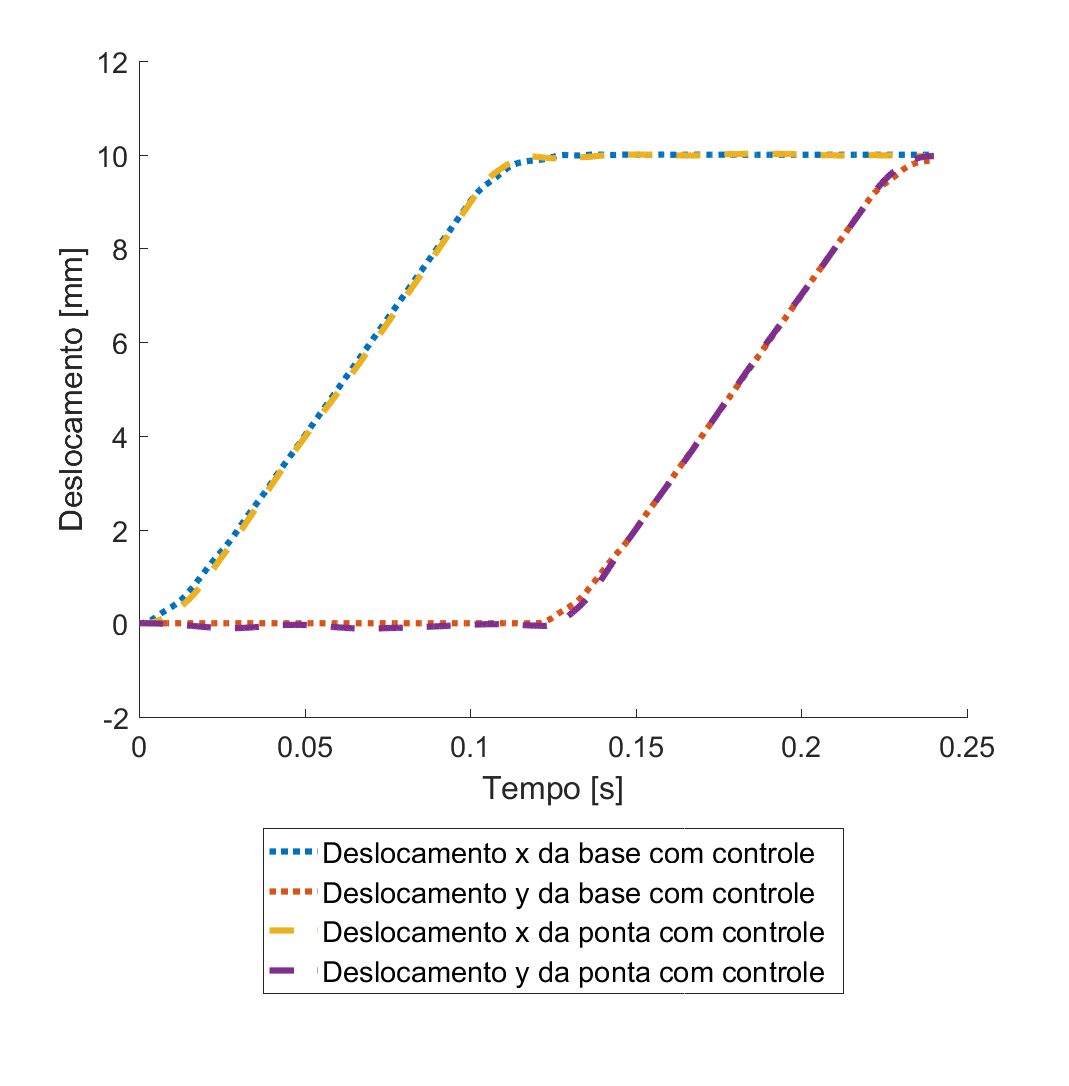
\includegraphics[width=0.38\textwidth]{Sim 1B_des_c.png}
        \label{fig:1B_des_c}
    }
  \end{figure}
\end{frame}


\subsection{\insertsectionnumber .\insertsubsectionnumber . Resultados da Simulação - Variação do Coeficiente de Amortecimento}

\begin{frame}
  \frametitle{\insertsubsection}
  \begin{figure}[H]
    \centering
    \caption{Caminhos da ponta e da base.}
    \subfigure[Sem controle.]{
        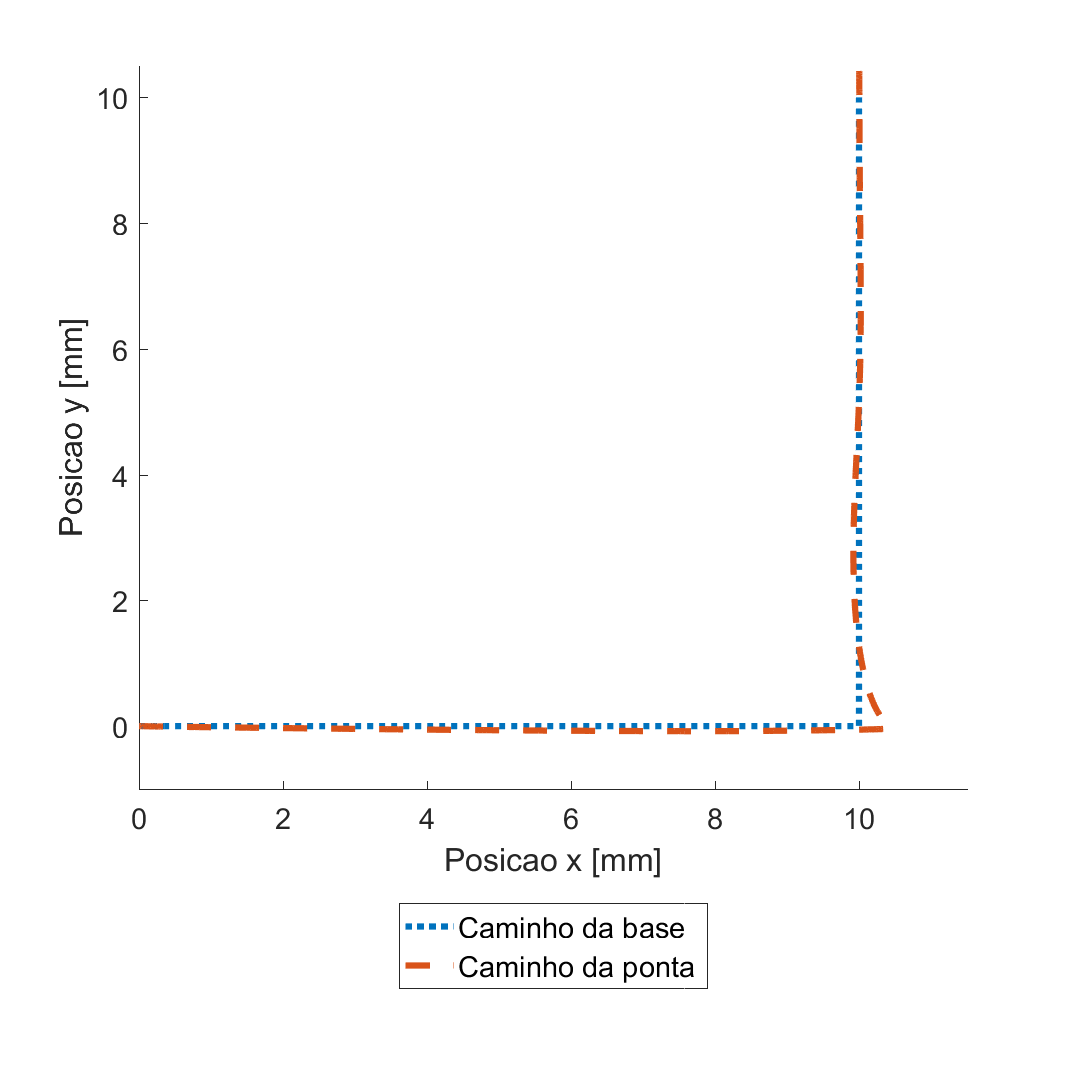
\includegraphics[width=0.38\textwidth]{Sim ref_cam_s.png}
        \label{fig:ref_cam_s}
    }
    \hfill
    \subfigure[Com controle.]{
        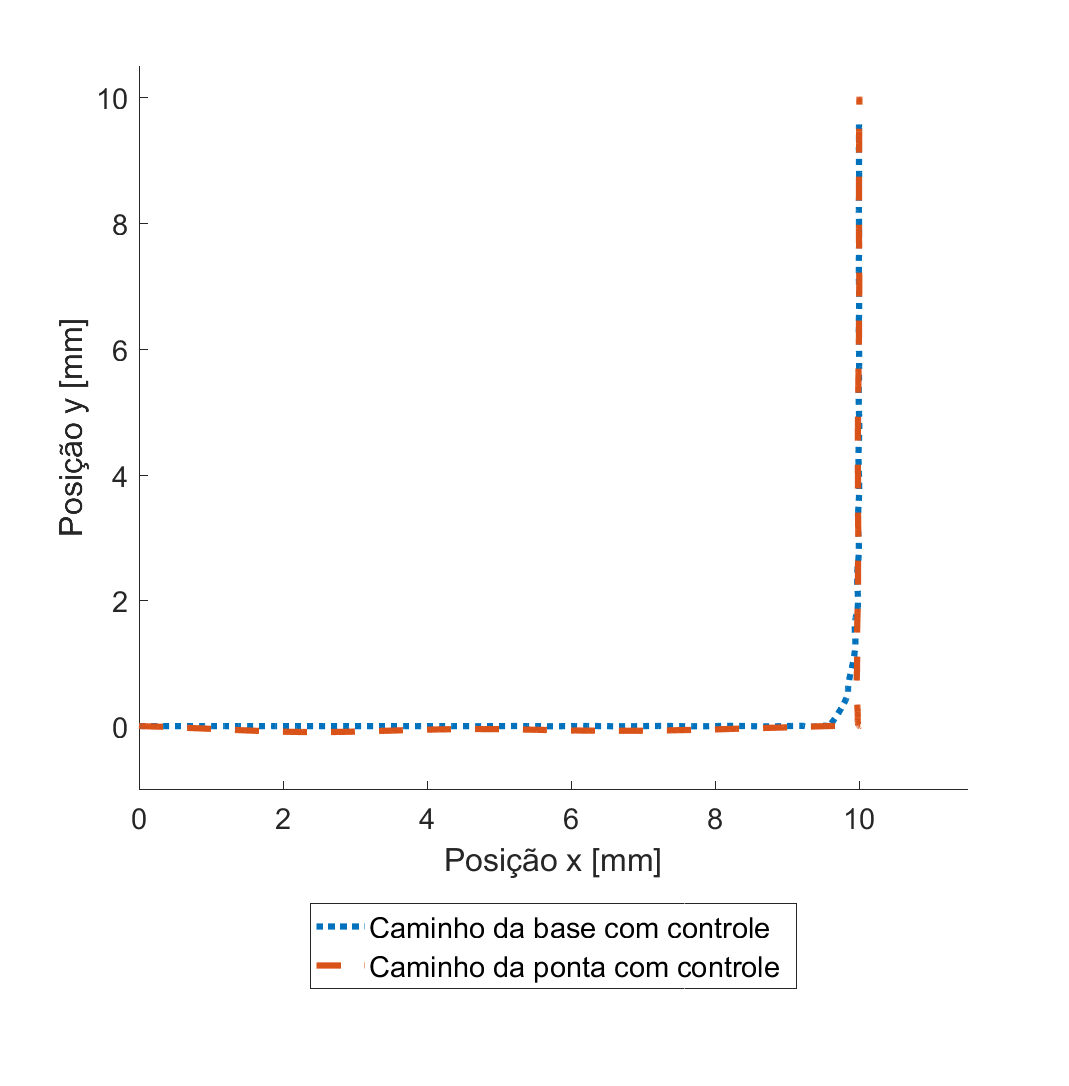
\includegraphics[width=0.38\textwidth]{Sim ref_cam_c.png}
        \label{fig:ref_cam_c}
    }
  \end{figure}
\end{frame}

\begin{frame}
  \frametitle{\insertsubsection}
  \begin{figure}[H]
    \centering
    \caption{Caminhos da ponta e da base - Detalhamento}
    \subfigure[Sem controle.]{
        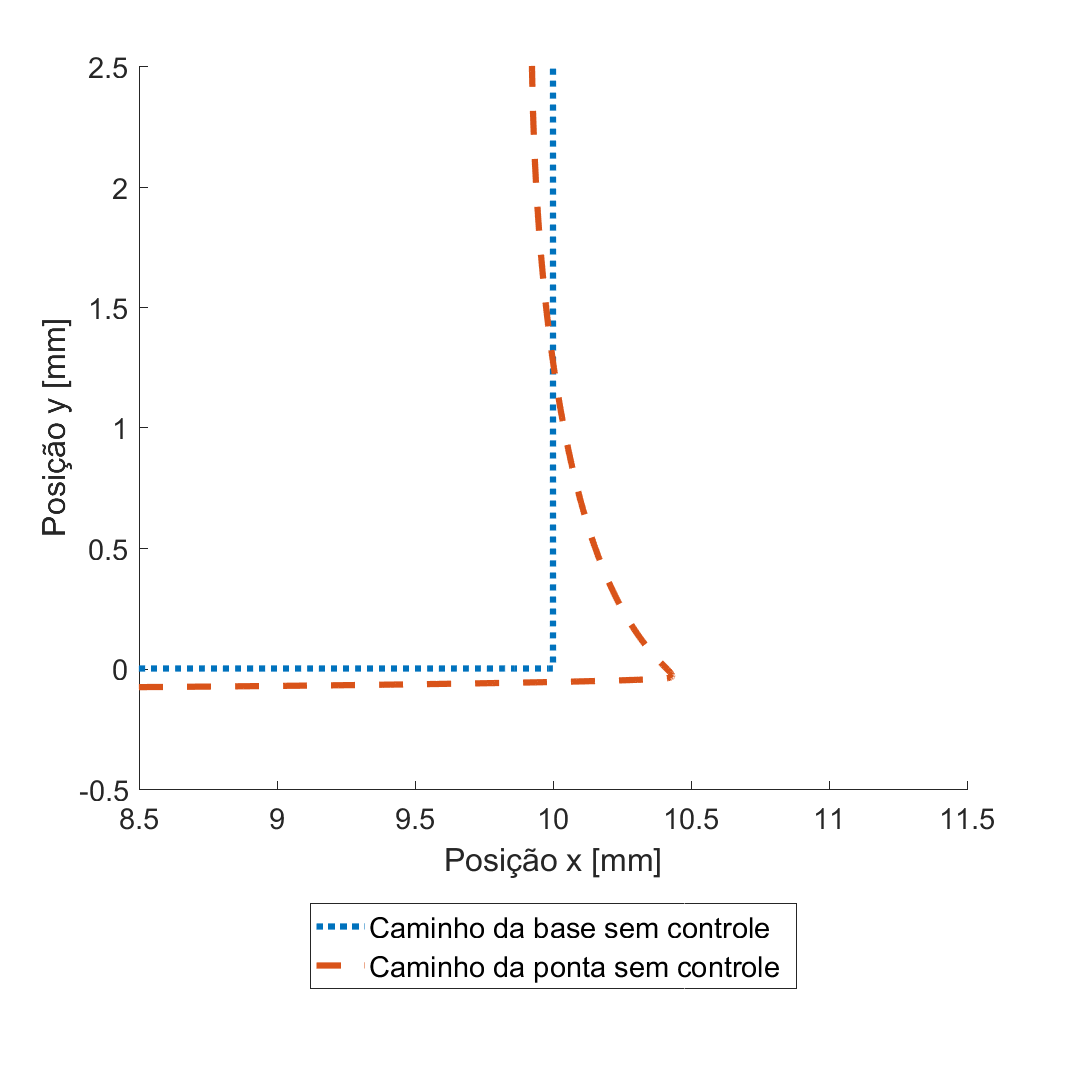
\includegraphics[width=0.38\textwidth]{Sim ref_cam_s_zoom.png}
        \label{fig:ref_cam_s_zoom}
    }
    \hfill
    \subfigure[Com controle.]{
        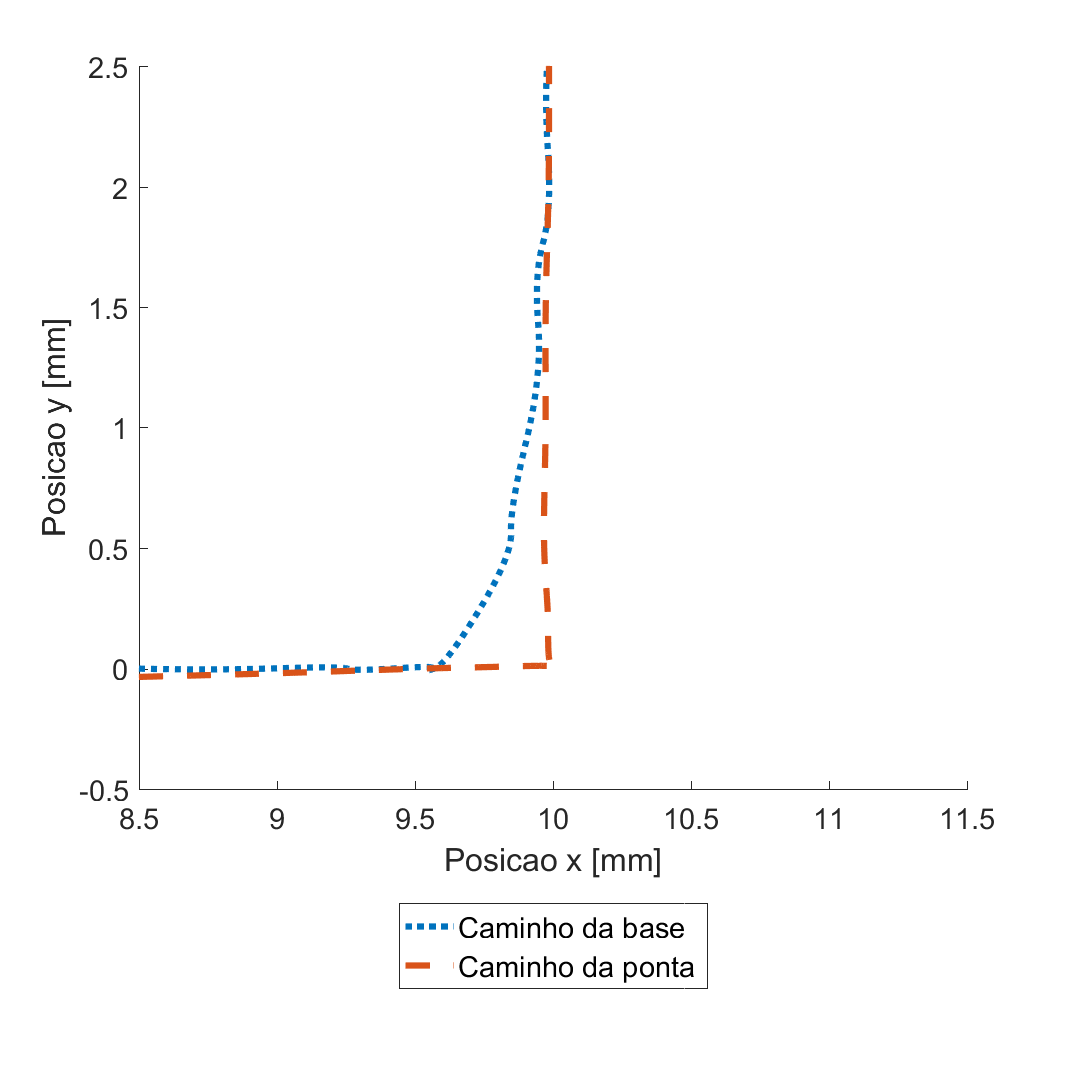
\includegraphics[width=0.38\textwidth]{Sim ref_cam_c_zoom.png}
        \label{fig:ref_cam_c_zoom}
    }
  \end{figure}
\end{frame}

\begin{frame}
  \frametitle{\insertsubsection}
  \begin{figure}[H]
    \centering
    \caption{Deslocamentos da ponta e da base.}
    \subfigure[Sem controle.]{
        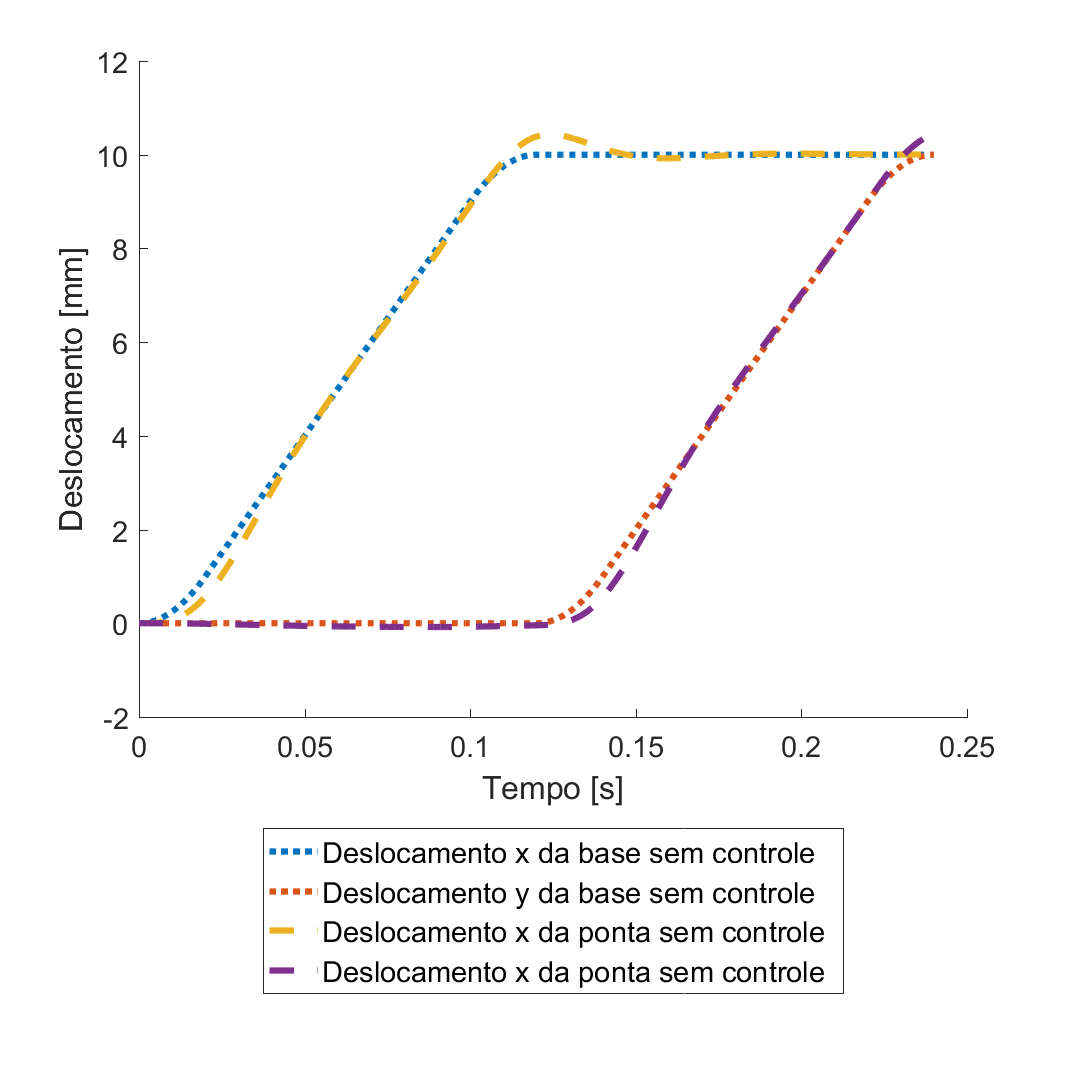
\includegraphics[width=0.38\textwidth]{Sim ref_des_s.png}
        \label{fig:ref_des_s}
    }
    \hfill
    \subfigure[Com controle.]{
        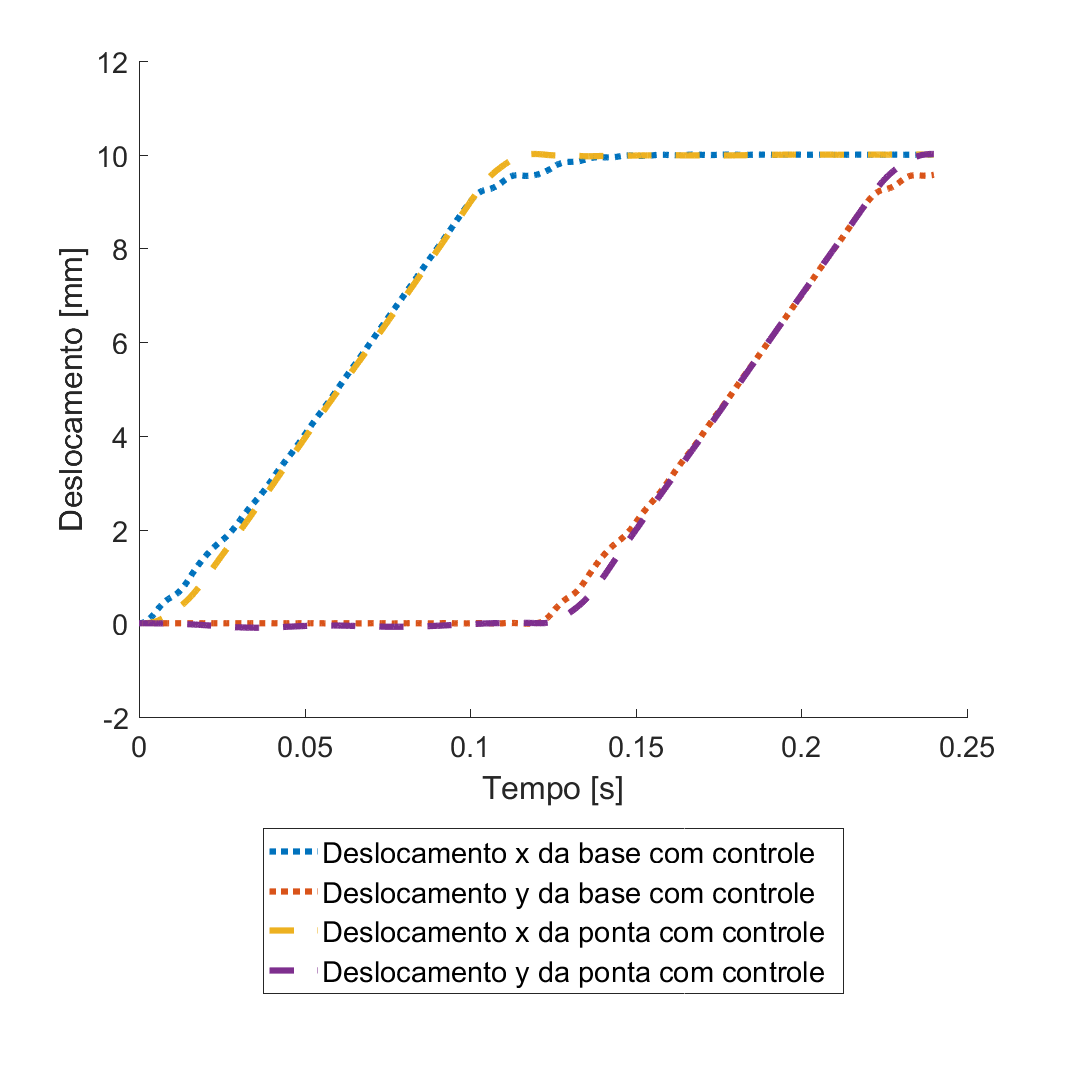
\includegraphics[width=0.38\textwidth]{Sim ref_des_c.png}
        \label{fig:ref_des_c}
    }
    \label{fig:ref_des}
  \end{figure}
\end{frame}

\begin{frame}
  \frametitle{\insertsubsection}
  \begin{figure}[H]
    \centering
    \caption{Velocidades da ponta e da base.}
    \subfigure[Sem controle.]{
        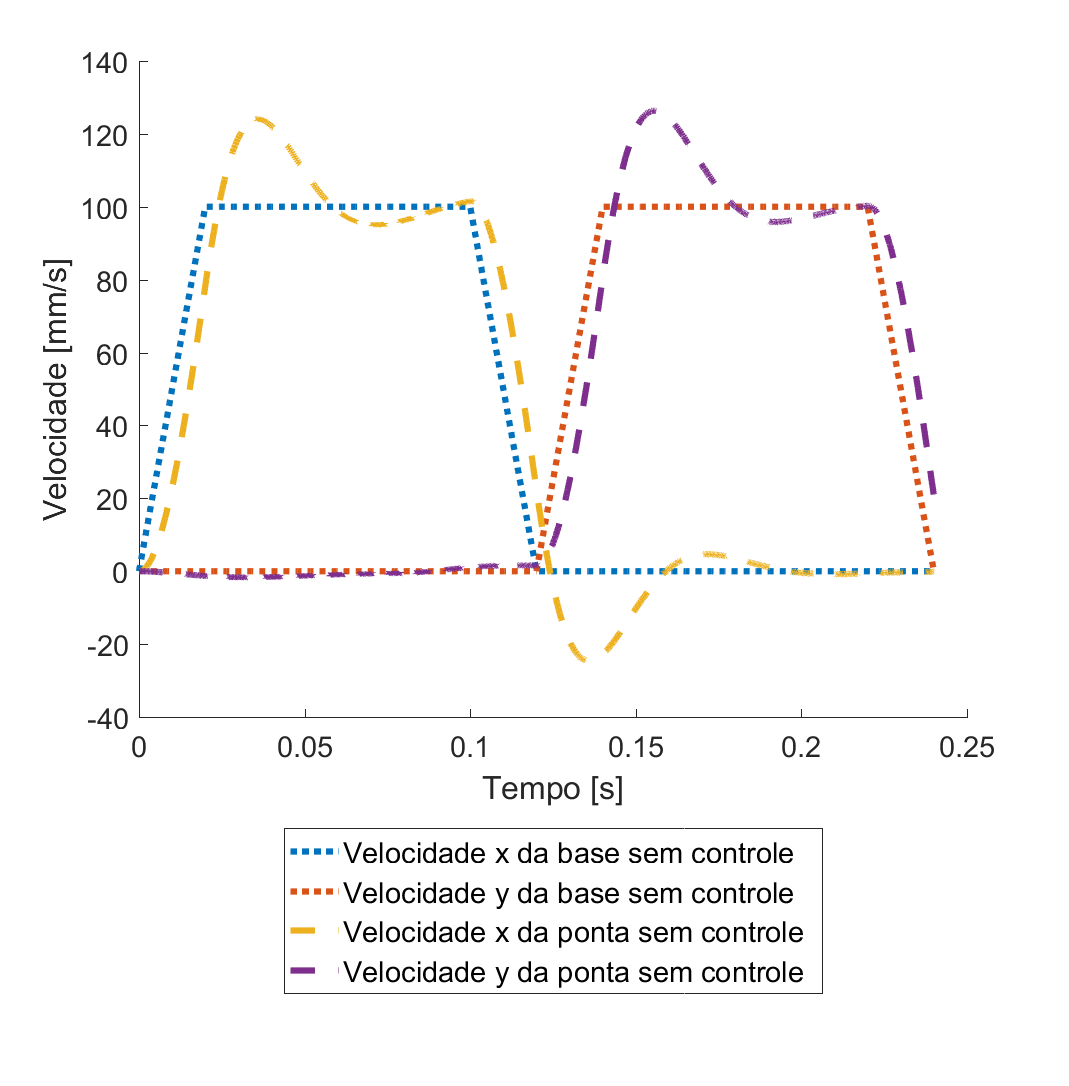
\includegraphics[width=0.38\textwidth]{Sim ref_vel_s.png}
        \label{fig:ref_vel_s}
    }
    \hfill
    \subfigure[Com controle.]{
        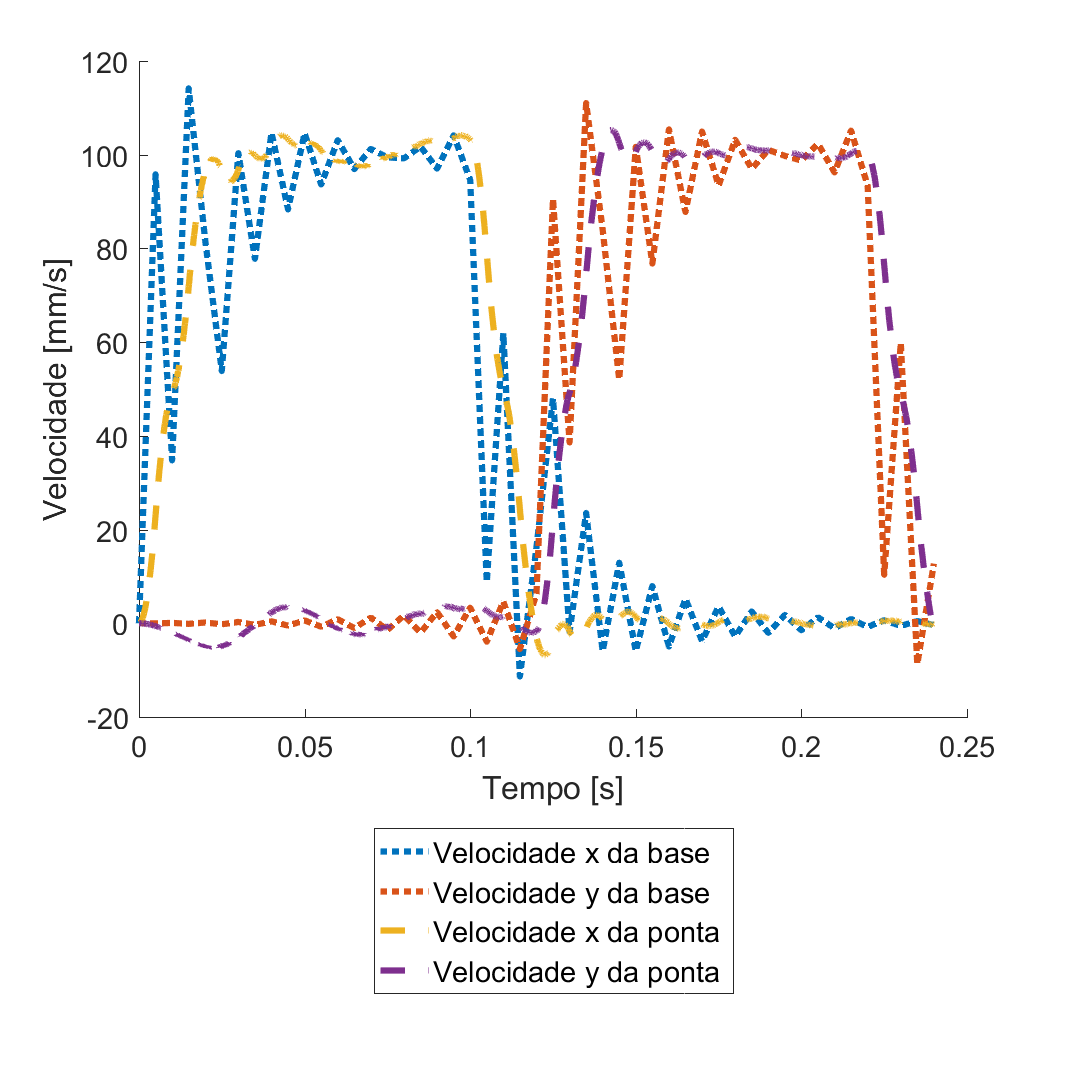
\includegraphics[width=0.38\textwidth]{Sim ref_vel_c.png}
        \label{fig:ref_vel_c}
    }
    \label{fig:ref_vel}
  \end{figure}
\end{frame}

\subsection{\insertsectionnumber .\insertsubsectionnumber . Resultados da Simulação - Variação na Aceleração}

\begin{frame}
  \frametitle{\insertsubsection}
  \begin{figure}[H]
    \centering
    \caption{Caminhos da ponta e da base.}
    \subfigure[Sem controle.]{
        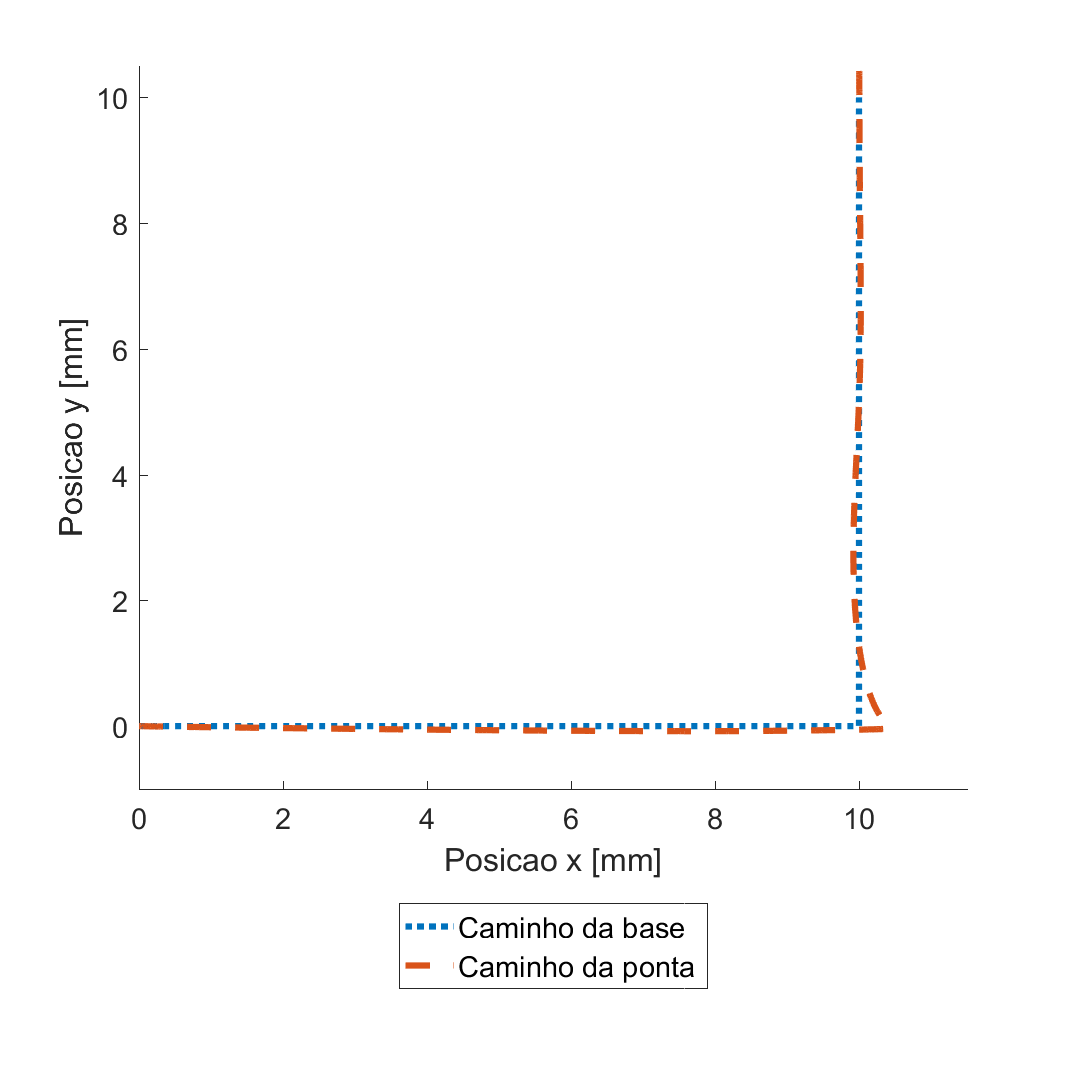
\includegraphics[width=0.38\textwidth]{Sim ref_cam_s.png}
        \label{fig:ref_cam_s}
    }
    \hfill
    \subfigure[Com controle.]{
        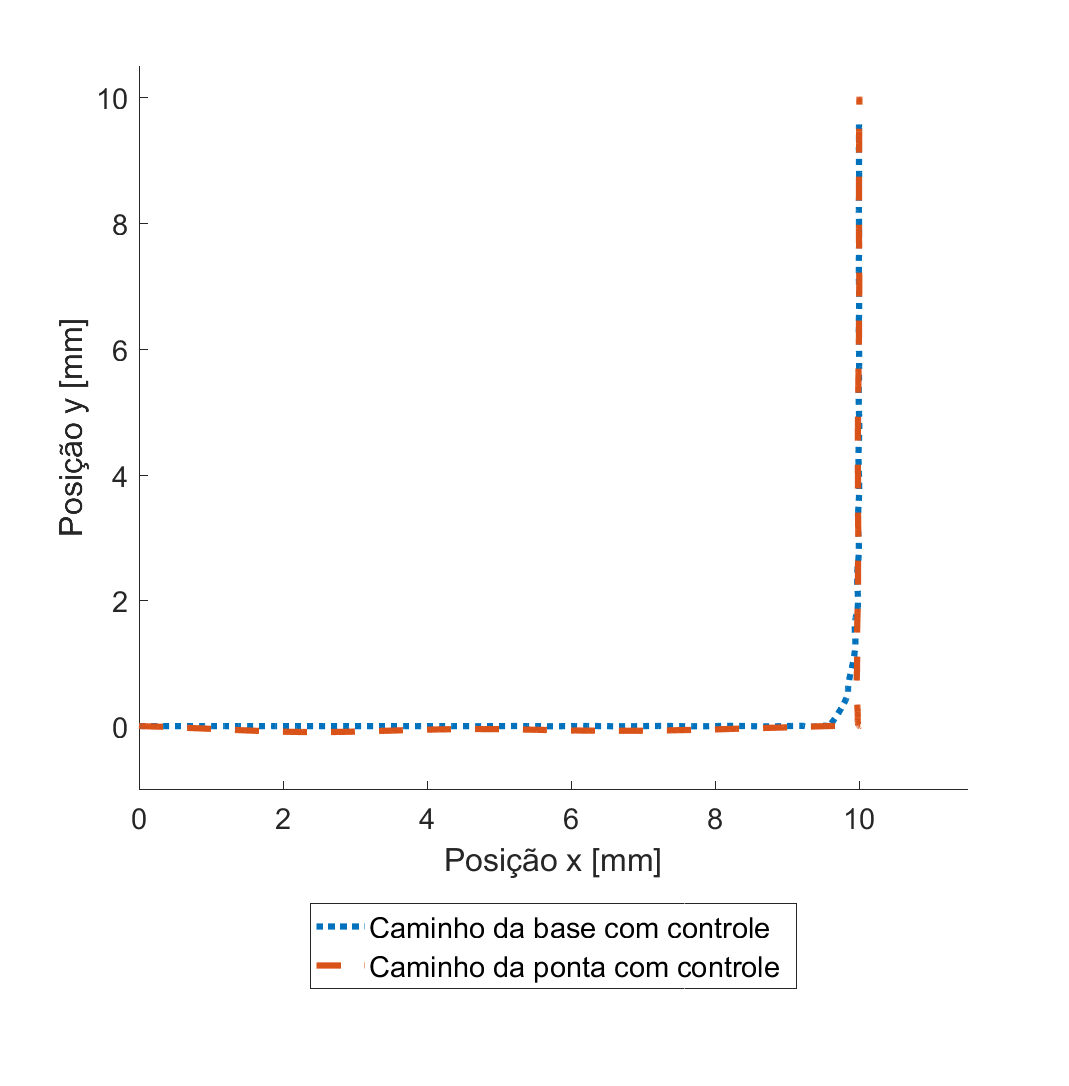
\includegraphics[width=0.38\textwidth]{Sim ref_cam_c.png}
        \label{fig:ref_cam_c}
    }
  \end{figure}
\end{frame}

\begin{frame}
  \frametitle{\insertsubsection}
  \begin{figure}[H]
    \centering
    \caption{Caminhos da ponta e da base - Detalhamento}
    \subfigure[Sem controle.]{
        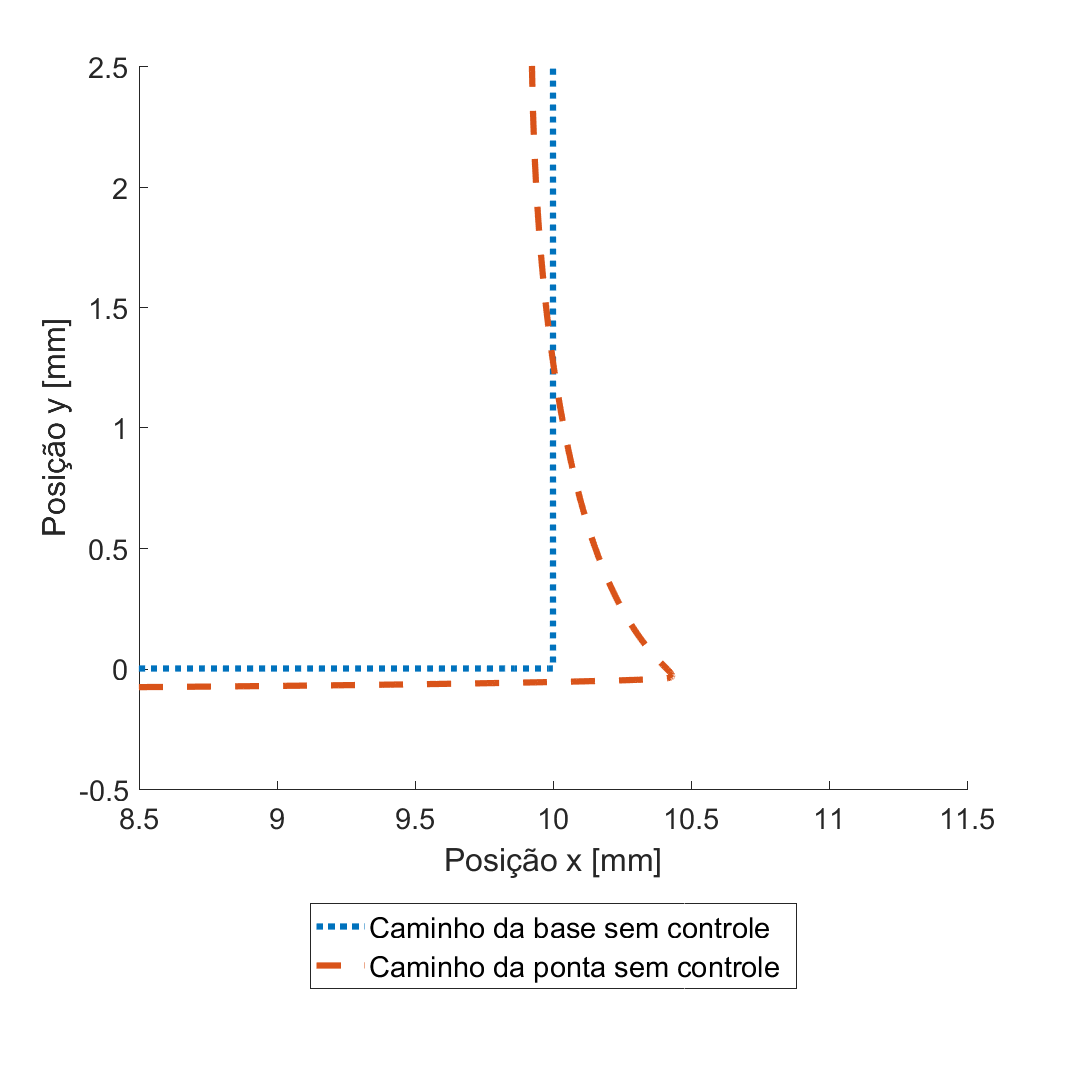
\includegraphics[width=0.38\textwidth]{Sim ref_cam_s_zoom.png}
        \label{fig:ref_cam_s_zoom}
    }
    \hfill
    \subfigure[Com controle.]{
        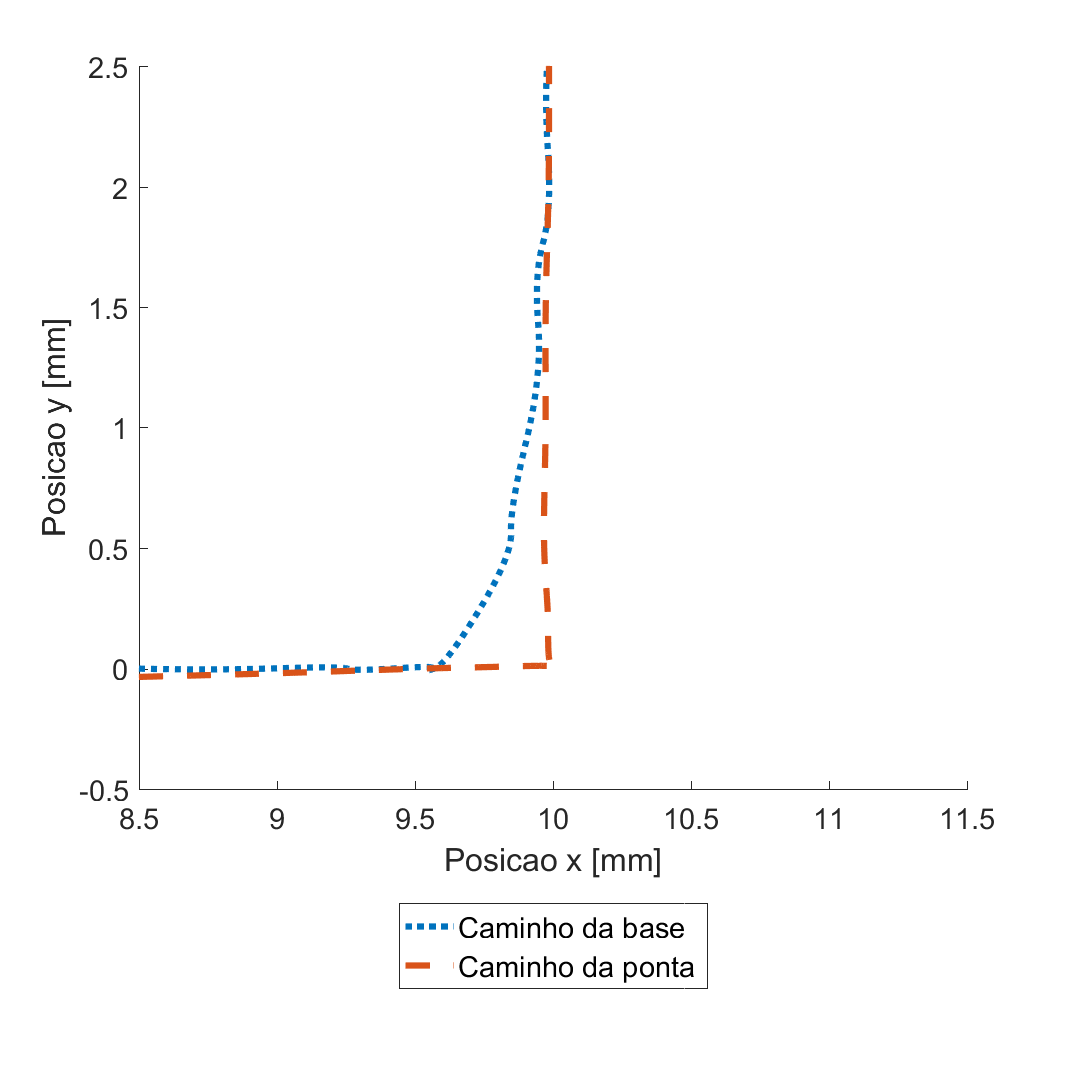
\includegraphics[width=0.38\textwidth]{Sim ref_cam_c_zoom.png}
        \label{fig:ref_cam_c_zoom}
    }
  \end{figure}
\end{frame}

\begin{frame}
  \frametitle{\insertsubsection}
  \begin{figure}[H]
    \centering
    \caption{Deslocamentos da ponta e da base.}
    \subfigure[Sem controle.]{
        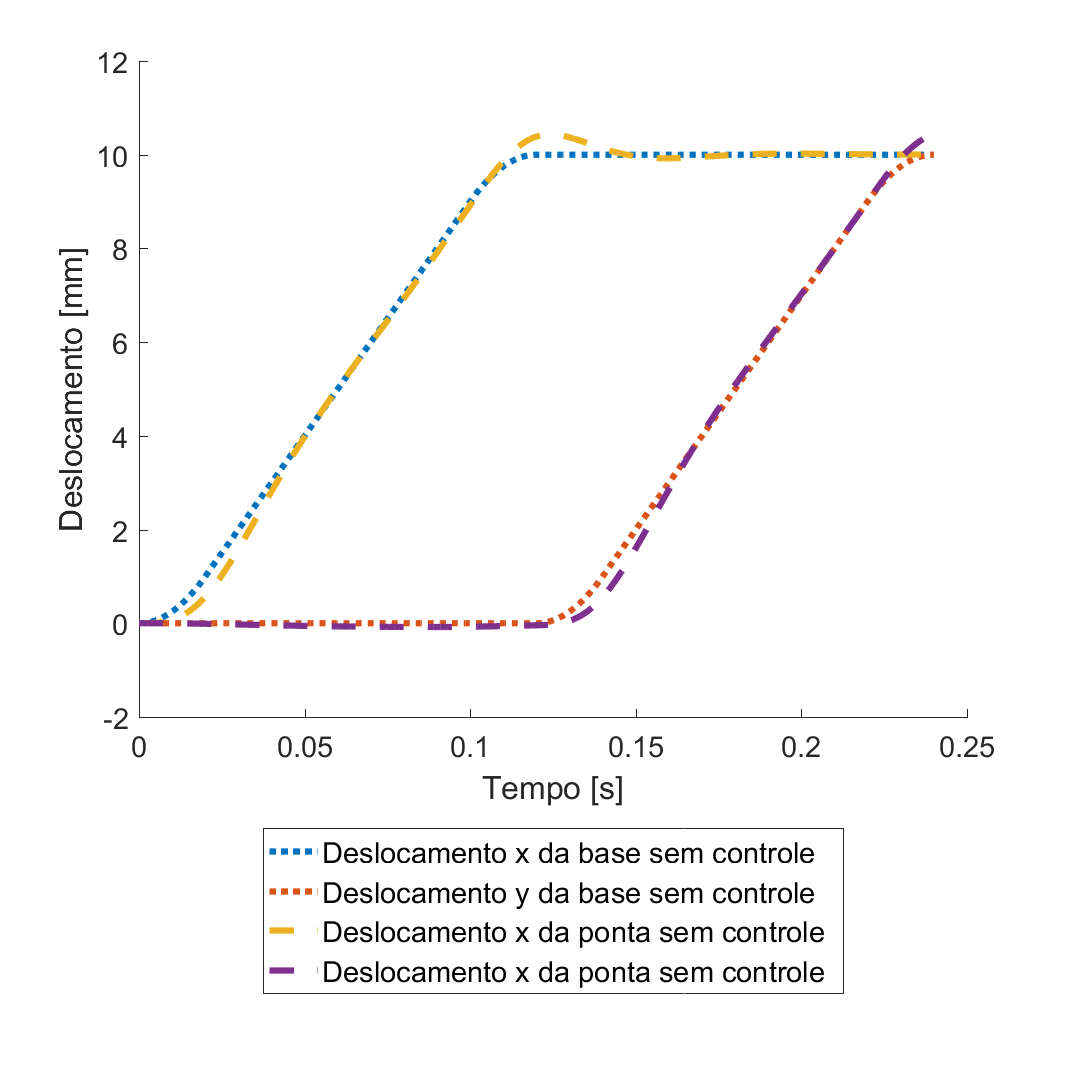
\includegraphics[width=0.38\textwidth]{Sim ref_des_s.png}
        \label{fig:ref_des_s}
    }
    \hfill
    \subfigure[Com controle.]{
        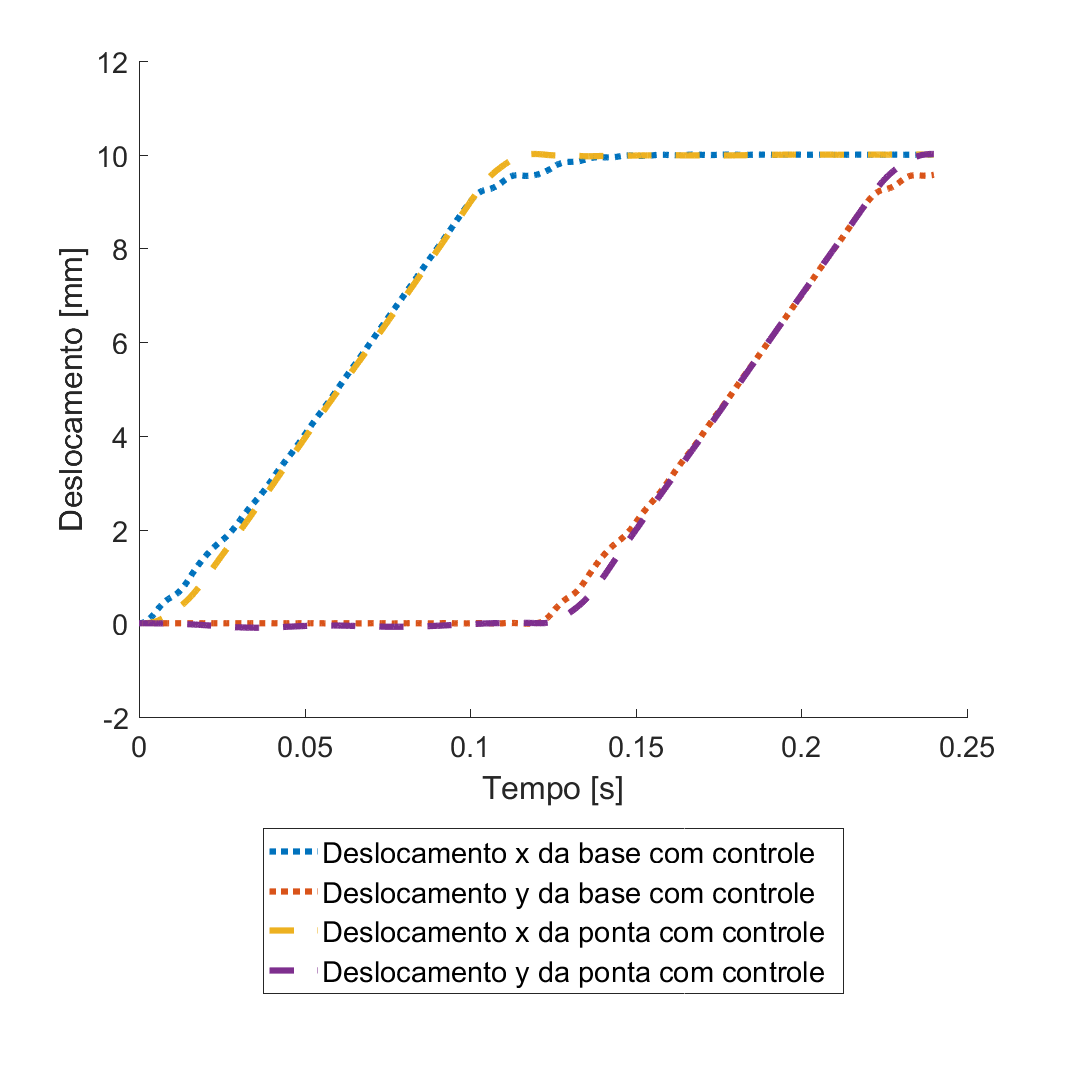
\includegraphics[width=0.38\textwidth]{Sim ref_des_c.png}
        \label{fig:ref_des_c}
    }
    \label{fig:ref_des}
  \end{figure}
\end{frame}

\begin{frame}
  \frametitle{\insertsubsection}
  \begin{figure}[H]
    \centering
    \caption{Velocidades da ponta e da base.}
    \subfigure[Sem controle.]{
        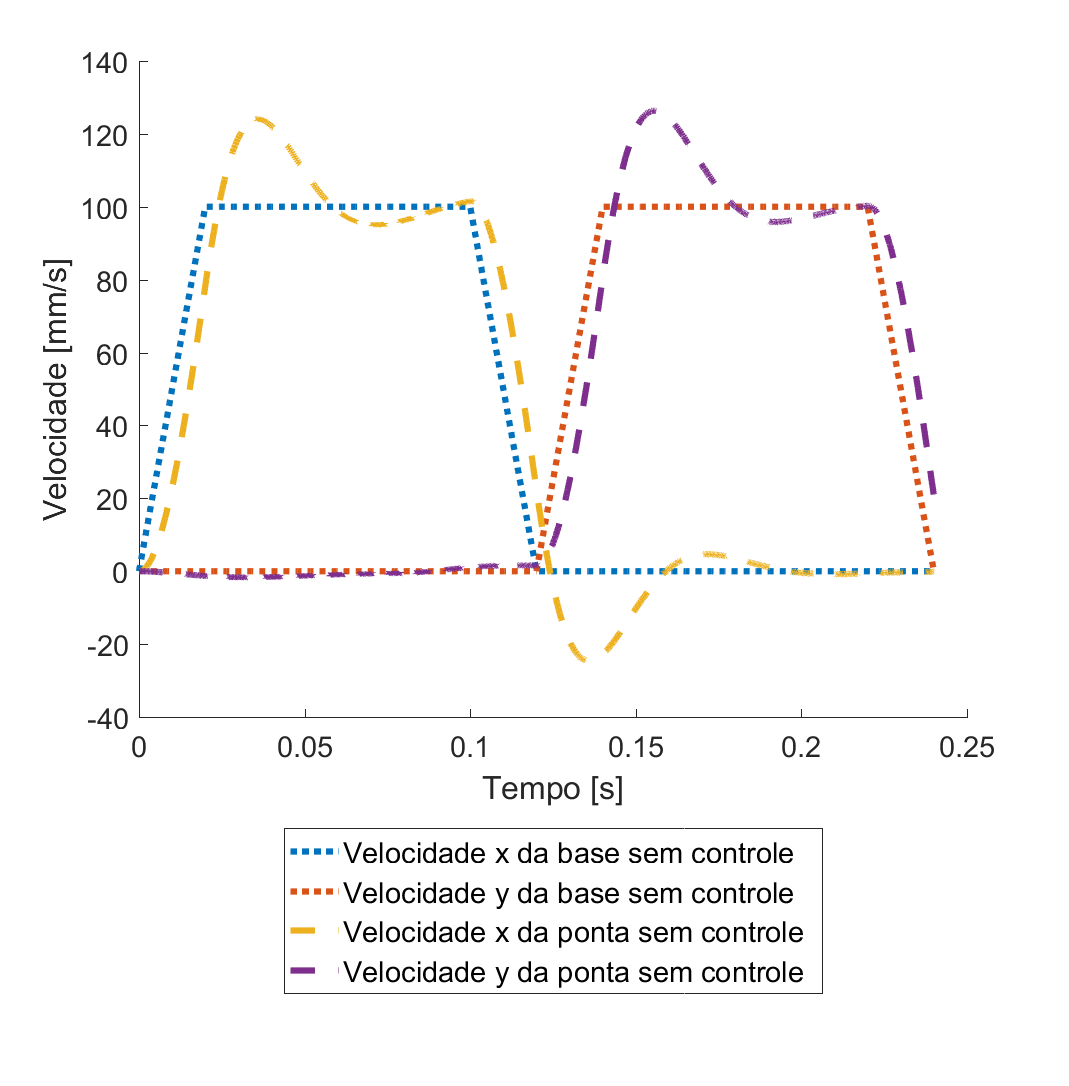
\includegraphics[width=0.38\textwidth]{Sim ref_vel_s.png}
        \label{fig:ref_vel_s}
    }
    \hfill
    \subfigure[Com controle.]{
        \includegraphics[width=0.38\textwidth]{Sim ref_vel_c.png}
        \label{fig:ref_vel_c}
    }
    \label{fig:ref_vel}
  \end{figure}
\end{frame}

\subsection{\insertsectionnumber .\insertsubsectionnumber . Resultados da Simulação - Variação da Velocidade desejada}

\begin{frame}
  \frametitle{\insertsubsection}
  \begin{figure}[H]
    \centering
    \caption{Caminhos da ponta e da base.}
    \subfigure[Sem controle.]{
        \includegraphics[width=0.38\textwidth]{Sim ref_cam_s.png}
        \label{fig:ref_cam_s}
    }
    \hfill
    \subfigure[Com controle.]{
        \includegraphics[width=0.38\textwidth]{Sim ref_cam_c.png}
        \label{fig:ref_cam_c}
    }
  \end{figure}
\end{frame}

\begin{frame}
  \frametitle{\insertsubsection}
  \begin{figure}[H]
    \centering
    \caption{Caminhos da ponta e da base - Detalhamento}
    \subfigure[Sem controle.]{
        \includegraphics[width=0.38\textwidth]{Sim ref_cam_s_zoom.png}
        \label{fig:ref_cam_s_zoom}
    }
    \hfill
    \subfigure[Com controle.]{
        \includegraphics[width=0.38\textwidth]{Sim ref_cam_c_zoom.png}
        \label{fig:ref_cam_c_zoom}
    }
  \end{figure}
\end{frame}

\begin{frame}
  \frametitle{\insertsubsection}
  \begin{figure}[H]
    \centering
    \caption{Deslocamentos da ponta e da base.}
    \subfigure[Sem controle.]{
        \includegraphics[width=0.38\textwidth]{Sim ref_des_s.png}
        \label{fig:ref_des_s}
    }
    \hfill
    \subfigure[Com controle.]{
        \includegraphics[width=0.38\textwidth]{Sim ref_des_c.png}
        \label{fig:ref_des_c}
    }
    \label{fig:ref_des}
  \end{figure}
\end{frame}

\begin{frame}
  \frametitle{\insertsubsection}
  \begin{figure}[H]
    \centering
    \caption{Velocidades da ponta e da base.}
    \subfigure[Sem controle.]{
        \includegraphics[width=0.38\textwidth]{Sim ref_vel_s.png}
        \label{fig:ref_vel_s}
    }
    \hfill
    \subfigure[Com controle.]{
        \includegraphics[width=0.38\textwidth]{Sim ref_vel_c.png}
        \label{fig:ref_vel_c}
    }
    \label{fig:ref_vel}
  \end{figure}
\end{frame}

\subsection{\insertsectionnumber .\insertsubsectionnumber . Resultados da Simulação - Variação do Passo de tempo}

\begin{frame}
  \frametitle{\insertsubsection}
  \begin{figure}[H]
    \centering
    \caption{Caminhos da ponta e da base.}
    \subfigure[Sem controle.]{
        \includegraphics[width=0.38\textwidth]{Sim ref_cam_s.png}
        \label{fig:ref_cam_s}
    }
    \hfill
    \subfigure[Com controle.]{
        \includegraphics[width=0.38\textwidth]{Sim ref_cam_c.png}
        \label{fig:ref_cam_c}
    }
  \end{figure}
\end{frame}

\begin{frame}
  \frametitle{\insertsubsection}
  \begin{figure}[H]
    \centering
    \caption{Caminhos da ponta e da base - Detalhamento}
    \subfigure[Sem controle.]{
        \includegraphics[width=0.38\textwidth]{Sim ref_cam_s_zoom.png}
        \label{fig:ref_cam_s_zoom}
    }
    \hfill
    \subfigure[Com controle.]{
        \includegraphics[width=0.38\textwidth]{Sim ref_cam_c_zoom.png}
        \label{fig:ref_cam_c_zoom}
    }
  \end{figure}
\end{frame}

\begin{frame}
  \frametitle{\insertsubsection}
  \begin{figure}[H]
    \centering
    \caption{Deslocamentos da ponta e da base.}
    \subfigure[Sem controle.]{
        \includegraphics[width=0.38\textwidth]{Sim ref_des_s.png}
        \label{fig:ref_des_s}
    }
    \hfill
    \subfigure[Com controle.]{
        \includegraphics[width=0.38\textwidth]{Sim ref_des_c.png}
        \label{fig:ref_des_c}
    }
    \label{fig:ref_des}
  \end{figure}
\end{frame}

\begin{frame}
  \frametitle{\insertsubsection}
  \begin{figure}[H]
    \centering
    \caption{Velocidades da ponta e da base.}
    \subfigure[Sem controle.]{
        \includegraphics[width=0.38\textwidth]{Sim ref_vel_s.png}
        \label{fig:ref_vel_s}
    }
    \hfill
    \subfigure[Com controle.]{
        \includegraphics[width=0.38\textwidth]{Sim ref_vel_c.png}
        \label{fig:ref_vel_c}
    }
    \label{fig:ref_vel}
  \end{figure}
\end{frame}

\section{\insertsectionnumber . Conclusão}

\begin{frame}
  \frametitle{\insertsection}
  \begin{itemize}
    \item conclusao
    \item conclusao
    \item conclusao
  \end{itemize}
\end{frame}

% Remove a logo para o próximo slide
\setbeamertemplate{logo}{}
\begin{frame}
    
  \backgroundlogo
  \begin{center}
    \huge{Obrigado!}
  \end{center}
\end{frame}

\bibliographystyle{abntex2-alf}      
\bibliography{referencias}	

\end{document}